\documentclass{article}
\usepackage{dsfont}

\usepackage[utf8]{inputenc}
\usepackage[spanish,mexico]{babel}
\usepackage[margin=2.5cm]{geometry}
\usepackage{graphicx}
\usepackage{float}
\usepackage{dsfont}
\usepackage[export]{adjustbox}
\usepackage{caption}
\usepackage{subcaption}
\usepackage{amsmath,amssymb}
\usepackage{recycle}
\usepackage{amsfonts}
\usepackage{amsthm}
\usepackage{listings}
\usepackage{fancyhdr}
\usepackage{comment}
\usepackage[backend=biber, style=numeric]{biblatex}
\addbibresource{contenido/references.bib}
\pagestyle{fancy}
\fancyhf{}
\graphicspath{{./imagenes/}}
\usepackage{background}
\usepackage{tcolorbox}
\usepackage{hyperref}
\hypersetup{
    colorlinks=true,
    citecolor=black,
    linktoc=all,
    linkcolor=black,
    urlcolor=blue
}
\usepackage{algorithm}
\usepackage[noend]{algpseudocode}
\newtheorem{theorem}{Theorem}[section]
\usepackage{setspace}
\usepackage{parskip}
\setlength{\parskip}{10pt}
\usepackage{longtable}
\usepackage{xcolor}

\definecolor{codegreen}{rgb}{0,0.6,0}
\definecolor{codegray}{rgb}{0.5,0.5,0.5}
\definecolor{codepurple}{rgb}{0.58,0,0.82}
\definecolor{backcolour}{rgb}{0.95,0.95,0.92}

\lstdefinestyle{mystyle}{
    backgroundcolor=\color{backcolour},
    commentstyle=\color{codegreen},
    keywordstyle=\color{magenta},
    numberstyle=\tiny\color{codegray},
    stringstyle=\color{codepurple},
    basicstyle=\ttfamily\footnotesize,
    breakatwhitespace=false,
    breaklines=true,
    captionpos=b,
    keepspaces=true,
    numbers=left,
    numbersep=5pt,
    showspaces=false,
    showstringspaces=false,
    showtabs=false,
    tabsize=2
}

\lstset{style=mystyle}

\lstset{
     literate=%
         {á}{{\'a}}1
         {í}{{\'i}}1
         {é}{{\'e}}1
         {ý}{{\'y}}1
         {ú}{{\'u}}1
         {ó}{{\'o}}1
         {ñ}{{\~n}}1
         {ě}{{\v{e}}}1
         {š}{{\v{s}}}1
         {č}{{\v{c}}}1
         {ř}{{\v{r}}}1
         {ž}{{\v{z}}}1
         {ď}{{\v{d}}}1
         {ť}{{\v{t}}}1
         {ň}{{\v{n}}}1
         {ů}{{\r{u}}}1
         {Á}{{\'A}}1
         {Í}{{\'I}}1
         {É}{{\'E}}1
         {Ý}{{\'Y}}1
         {Ú}{{\'U}}1
         {Ó}{{\'O}}1
         {Ě}{{\v{E}}}1
         {Š}{{\v{S}}}1
         {Č}{{\v{C}}}1
         {Ř}{{\v{R}}}1
         {Ž}{{\v{Z}}}1
         {Ď}{{\v{D}}}1
         {Ť}{{\v{T}}}1
         {Ň}{{\v{N}}}1
         {Ů}{{\r{U}}}1
         {²}{{$^2$}}1
} % Se agregan los paquetes utilizados en el documento.
\input{estructura/estilo} % Define la marca de agua, encabezado y pie de página.


\begin{document}

\begin{titlepage}
\centering
{\Large UNIVERSIDAD NACIONAL AUTÓNOMA DE MÉXICO  \par}
\vspace{.3cm}
{\Large FACULTAD DE CIENCIAS \par}
\begin{figure}[h]
	   \minipage{0.76\textwidth}
			
\includegraphics[width=3.5cm]{imagenes/Logo_UNAM.png}
			\label{EscudoUNAM}
	   \endminipage
	   \minipage{0.32\textwidth}
			
\includegraphics[height = 4.4cm ,width=4cm]{imagenes/Logo_FC.png}
			\label{EscudoFC}
		\endminipage
	\end{figure}
\vfill
\noindent\hrulefill \\
{\scshape\Huge
Almacenes y Minería de Datos\par} %Título
\vspace{0.5cm}
{\scshape\Large Proyecto Final - Minería de Datos Aplicada a México
 \par}
\vspace{0.5cm}
\noindent\hrulefill \\
\vfill

\begin{center}
    \Large
    \textbf{Alumnos:}

    \vspace{.3cm}
    \large	\begin{itemize}
        \item Méndez Ávila Luis Geovanni \quad 317143980
        \item Paredes Zamudio Luis Daniel \quad 318159926
        \item Sánchez Rosas Roberto Samuel \quad 318355159
    \end{itemize}

\end{center}

\vfill
{\Large \textbf{Profesora:} L. en C.C. Jessica Santizo Galicia \\
             \par}
\vfill
{\large 10 de Junio de 2026 \par}
\end{titlepage}
\setcounter{page}{1}
\newpage
\newpage

\tableofcontents
\newpage

\begin{spacing}{1.5}
    \section{Introducción: Análisis de la Incidencia Delictiva Estatal}

No es noticia nueva de que México sufre de un serio problema de delicuencia. Y esto, desgraciadamente,
no ha disminuido considerablemente en 10 años a la fecha. Pero la realidad es que distntos estados
de la república sufren de delitos en particular que, aunque presentes en otros lugares, no son el
principal foco del lugar.

Nuestro objetivo al analizar la incidencia delectiva es poder identificar no solo cuales son éstos
delitos los más preliminares en cada estado, si no también poder crear un modelo que establezca cual
es delito más probable que pueda sufrir un ciudadano de un estado en particular.

Desgraciadamente, todxs somos propensos a sufrirlos, pero identificarlos no solo nos permite a nostros
como habitantes poder prepararnos para evitarlos lo más que se pueda, como le puede servir a las autoridades
componentes para concientizar y, utópicamente, idear soluciones que reduzcan verdaderamente la epidemia
de delicuencia que sufre el país.

Este dataset pertenece a la \href{https://www.datos.gob.mx/}{Plataforma Nacional de Datos Abiertos Mexicana} y fue
creado por el Secretariado Ejecutivo del Sistema Nacional de Seguridad Pública (SESNSP). Este dataset, nombrado
simplemente como \textit{Incidencia Delictiva}, puede descargarse siguiendo \href{https://www.datos.gob.mx/dataset/incidencia_delictiva/resource/d9b2792a-33a2-4ea8-8527-210d9e99de5e}{este enlace}.

    \section{Análisis Exploratorio de Datos}

Haremos un análisis exploratorio para conocer el dataset en profundidad y poder identificar patrones, tendencias y relaciones entre las variables.
Esto nos permitirá tomar decisiones informadas sobre cómo abordar el problema de la incidencia delictiva más adelante en el proyecto,
principalmente para crear el modelo de predicción adecuado a este problema.

Para esto, haremos limpieza, análisis estadístico, detección de outliers y visualización de los datos.

Como mencionamos en la sección anterior, cada sección de este análisis se irá documentando con código y resultados, para pode seguir el
proceso de manera clara y transparente. De igual manera, el cuaderno de Jupyter con el código completo de este análisis se encuentra disponible
\href{https://github.com/wallsified/proyecto-final-aymdd/blob/yoba/modelo/notebooks/eda.ipynb}{aquí}, mientras que el código fuente de ésta
sección se encuentra disponible en \href{https://github.com/wallsified/proyecto-final-aymdd/tree/main/src/eda}{ésta carpeta} del repositorio
del proyecto.

\subsection{Diccionario de Datos}

\begin{lstlisting}[language=Python, caption={Código para generar el diccionario de datos}, label={lst:diccionario-datos}]
import sys
from pathlib import Path

# Resuelve el problema de las ubicaciones de los scripts
sys.path.insert(0, str(Path.cwd().parent))

import pandas as pd
import matplotlib.pyplot as plt
import seaborn as sns

from src import config
from src.data import DataRepository
from src.preprocessing import PreprocessingPipeline
from src.eda import StatisticsAnalyzer, OutlierDetector

# Tema visual por defecto del proyecto.
sns.set_theme(style=config.SEABORN_THEME, palette=config.PLOT_PALETTE)
pd.set_option("display.max_columns", 20)
pd.set_option("display.width", 140)
pd.set_option("display.max_colwidth", 200)

repo = DataRepository()
dataframe = repo.load()
repo.dictionary()
\end{lstlisting}

\begin{table}[ht]
  \centering
  \caption{Diccionario de datos}
  \small
  \resizebox{\textwidth}{!}{%
    \begin{tabular}{r l p{0.65\textwidth}}
      \hline
      \textbf{Índice} & \textbf{Nombre (tipo)} & \textbf{Descripción} \\
      \hline
      0 & \texttt{anio} (int64) & Año de registro de las averiguaciones previas y/o carpetas de investigación. \\
      1 & \texttt{clave\_ent} (int64) & Clave de la entidad, según el Marco Geoestadístico Nacional (MGN) del Instituto Nacional de Geografía y Estadística (INEGI). \\
      2 & \texttt{entidad} (str) & Entidad federativa de registro de las averiguaciones previas y/o carpetas de investigación. \\
      3 & \texttt{bien\_juridico\_afectado} (str) & Primera clasificación de los delitos en las averiguaciones previas y/o carpetas de investigación. (Patrimonio, vida, libertad, etc.) \\
      4 & \texttt{tipo\_delito} (str) & Segunda clasificación de los delitos. (Falsedad, Lesiones, Robo, etc.) \\
      5 & \texttt{subtipo\_delito} (str) & Tercera clasificación de los delitos. Subcategorías específicas de cada tipo de delito. (Lesiones dolosas, etc.). \\
      6 & \texttt{modalidad} (str) & Cuarta clasificación de los delitos. Forma en la que se comete el delito. (Con violencia, sin violencia, etc.) \\
      7 & \texttt{mes} (str) & Mes de registro de las averiguaciones previas y/o carpetas de investigación. \\
      8 & \texttt{fecha} (str) & Fecha de registro de las averiguaciones previas y/o carpetas de investigación. \\
      9 & \texttt{incidencia\_delictiva} (int64) & Incidencia delictiva del Fuero Común (Número absoluto de presuntos delitos registrados). \\
      10 & \texttt{entidad\_federativa} (str) & Entidad federativa de registro de las averiguaciones previas y/o carpetas de investigación. \\
      \hline
    \end{tabular}%
  }
  \label{tab:diccionario-datos}
\end{table}

\subsection{Overview del Dataset}

\begin{lstlisting}[language=Python, caption={Código para obtener un overview del dataset}, label={lst:overview-dataset}]
	dataframe
\end{lstlisting}

\begin{table}[ht]
  \centering
  \caption{Muestra del dataset: primeras filas}
  \scriptsize
  \resizebox{\textwidth}{!}{%
    \begin{tabular}{r r r l p{3.5cm} p{3cm} p{3cm} p{2.5cm} l l r l}
      \hline
      \textbf{idx} & \textbf{anio} & \textbf{clave\_ent} & \textbf{entidad} & \textbf{bien\_juridico\_afectado} & \textbf{tipo\_delito} & \textbf{subtipo\_delito} & \textbf{modalidad} & \textbf{mes} & \textbf{fecha} & \textbf{incidencia\_delictiva} & \textbf{entidad\_federativa} \\
      \hline
      0 & 2015 & 1 & Aguascalientes & El patrimonio & Abuso de confianza & Abuso de confianza & Abuso de confianza & Abril & 2015-04-01 & 22 & Aguascalientes \\
      1 & 2015 & 1 & Aguascalientes & El patrimonio & Abuso de confianza & Abuso de confianza & Abuso de confianza & Agosto & 2015-08-01 & 40 & Aguascalientes \\
      2 & 2015 & 1 & Aguascalientes & El patrimonio & Abuso de confianza & Abuso de confianza & Abuso de confianza & Diciembre & 2015-12-01 & 26 & Aguascalientes \\
      3 & 2015 & 1 & Aguascalientes & El patrimonio & Abuso de confianza & Abuso de confianza & Abuso de confianza & Enero & 2015-01-01 & 41 & Aguascalientes \\
      4 & 2015 & 1 & Aguascalientes & El patrimonio & Abuso de confianza & Abuso de confianza & Abuso de confianza & Febrero & 2015-02-01 & 33 & Aguascalientes \\
      \hline
    \end{tabular}%
  }
  \label{tab:dataset-head}
\end{table}

\begin{table}[ht]
  \centering
  \caption{Muestra del dataset: últimas filas}
  \scriptsize
  \resizebox{\textwidth}{!}{%
    \begin{tabular}{r r r l p{3.5cm} p{3cm} p{3cm} p{2.5cm} l l r l}
      \hline
      \textbf{idx} & \textbf{anio} & \textbf{clave\_ent} & \textbf{entidad} & \textbf{bien\_juridico\_afectado} & \textbf{tipo\_delito} & \textbf{subtipo\_delito} & \textbf{modalidad} & \textbf{mes} & \textbf{fecha} & \textbf{incidencia\_delictiva} & \textbf{entidad\_federativa} \\
      \hline
      413947 & 2025 & 32 & Zacatecas & Otros bienes jurídicos afectados (del fuero común) & Otros delitos del Fuero Común & Otros delitos del Fuero Común & Otros delitos del Fuero Común & Marzo & 2025-03-01 & 184 & Zacatecas \\
      413948 & 2025 & 32 & Zacatecas & Otros bienes jurídicos afectados (del fuero común) & Otros delitos del Fuero Común & Otros delitos del Fuero Común & Otros delitos del Fuero Común & Mayo & 2025-05-01 & 98 & Zacatecas \\
      413949 & 2025 & 32 & Zacatecas & Otros bienes jurídicos afectados (del fuero común) & Otros delitos del Fuero Común & Otros delitos del Fuero Común & Otros delitos del Fuero Común & Noviembre & 2025-11-01 & 92 & Zacatecas \\
      413950 & 2025 & 32 & Zacatecas & Otros bienes jurídicos afectados (del fuero común) & Otros delitos del Fuero Común & Otros delitos del Fuero Común & Otros delitos del Fuero Común & Octubre & 2025-10-01 & 99 & Zacatecas \\
      413951 & 2025 & 32 & Zacatecas & Otros bienes jurídicos afectados (del fuero común) & Otros delitos del Fuero Común & Otros delitos del Fuero Común & Otros delitos del Fuero Común & Septiembre & 2025-09-01 & 133 & Zacatecas \\
      \hline
    \end{tabular}%
  }
  \label{tab:dataset-tail}
\end{table}

El dataset contiene 413,952 registros que abarcan desde enero de 2015 hasta diciembre de 2025 (11 años).
Los datos están organizados a nivel estatal con granularidad mensual (32 entidades × 40+ tipos de delito × 132 meses),
lo que nos permite hacer análisis longitudinales de la evolución del delito en cada estado.

\subsection{Calidad y Limpieza de los Datos}

Haremos lo siguiente con el dataset original:

\begin{itemize}
  \item Borramos las columnas \texttt{anio} y \texttt{mes} para poder trabajar únicamente con fecha. Posteriormente, ésta última pasará a ser de tipo \texttt{datetime}.
  \item \texttt{entidad\_federativa} es un duplicado de \texttt{entidad}, por lo que borramos ésta columna.
  \item \texttt{clave\_entidad} no nos es de utilidad al ya tener el nombre de las entidades, por lo que borramos ésta columna.
  \item Analizamos el dataset en busca de duplicados y valores nulos.
  \item Consideraremos que una entrada es inválida si tiene valores NaN en \texttt{incidencia\_delictiva}, \texttt{fecha} y \texttt{entidad}. Una vez detectadas, serán eliminadas.
  \item Por revisión manual, vemos que algunos estados tienen su nombre completo, como \texttt{Veracruz de Ignacio de la Llave}. Acortaremos el nombre de estos estados para una visualización más limpia de la información.
\end{itemize}

\begin{lstlisting}[language=Python, caption={Código para limpiar el dataset}, label={lst:limpieza-dataset}]
cleaning_pipeline = PreprocessingPipeline(
    drop_columns=["anio", "clave_ent", "mes", "entidad_federativa"]
)
clean_dataset = cleaning_pipeline.run(dataframe)
# reorganizamos las columnas para tener la fecha como columna inicial del dataset
clean_dataset = clean_dataset.iloc[:, [5, 0, 1, 2, 3, 4, 6]]
cleaning_pipeline.save(clean_dataset)
\end{lstlisting}

\begin{lstlisting}
[1] Eliminando columnas declaradas en drop_columns
 Eliminadas: ['anio', 'clave_ent', 'mes', 'entidad_federativa']
[2] Convirtiendo '{self._date_col}' a datetime
   OK=413,952 / fallidos=0
 Rango: 2015-01-01 - 2025-12-01
[3] Eliminando filas con nulos en críticas
Filas: 413,952 - 413,952 (eliminadas: 0)
[4] Eliminando duplicados exactos
Filas: 413,952 - 413,952 (eliminadas: 0)
[5] Normalizando nombres de entidades federativas
413,952 filas x 7 columnas,
\end{lstlisting}

Vemos que, a pesar de ser un dataset de origen gubernamental, éste no contiene duplicados ni entradas inválidas. Por lo que solo se
realizó la conversión de fechas y la eliminación de las columnas con las que no trabajaremos.

\subsection{Estadísticas Descriptivas Numéricas}

En base a la naturaleza de nuestro dataset, el análisis estadístico se centrará principalmente en la variable \texttt{incidencia\_delictiva},
que representa el número de delitos reportados para cada combinación de estado, tipo de delito y fecha.

Veamos algunas estadísticas descriptivas clave para esta variable:

\begin{lstlisting}[language=Python, caption={Código para obtener estadísticas descriptivas numéricas}, label={lst:stats-descriptivas-numericas}]
# Carga del dataset limpio para análisis estadístico
repo = DataRepository("../data/processed/INM_estatal_dic25_clean.csv")
dataframe = repo.load()
stats = StatisticsAnalyzer(dataframe)
stats.numeric_stats()
\end{lstlisting}

\begin{table}[ht]
  \centering
  \caption{Estadísticas Descriptivas Numéricas}
  \scriptsize
  \resizebox{\textwidth}{!}{%
    \begin{tabular}{r r r l p{3.5cm} p{3cm} p{3cm} p{2.5cm} l l r l}
      \hline
      \textbf{idx} & \textbf{columna} & \textbf{Promedio} & \textbf{Mediana} & \textbf{Desviación Estándar} & \textbf{Valor Mínimo} & \textbf{Q1} & \textbf{Q3} & \textbf{Valor Máximo} & \textbf{Rango} \\
      0 & incidencia\_delictiva & 52.499106 & 2.0 & 204.518424 & 0.0 & 0.0 & 26.0 & 9968.0 & 9968.0 \\
      \hline
    \end{tabular}%
  }
  \label{tab:numeric-stats}
\end{table}

La media (52.5) es muy superior a la mediana (2.0), lo que indica un sesgo severo hacia la derecha. La mayoría de los registros
tienen baja incidencia (~2 delitos), pero algunos delitos registran valores enormes (siendo 9,968 el valor máximo). Sin embargo,
en un contexto real, la CDMX y el EdoMex son probablemente las entidades con valores más altos y más concentrados debido a su población
y urbanización. Validaremos esto más adelante.

En ese sentido, esto no sería (necesariamente) un sesgo en los datos, si no que refleja disparidades geográficas genuinas en la delincuencia.
Sin embargo, eso no significa que, nuevamente en un contexto real, no se reporte de la misma manera en otros estados.

\subsubsection{Histogramas de incidencia delictiva}

\begin{lstlisting}[language=Python, caption={Código para generar histogramas de incidencia delictiva}, label={lst:histogramas-incidencia-delictiva}]
fig, axes = plt.subplots(2, 1, figsize=(10, 12))

sns.histplot(
    data=dataframe,
    x="incidencia_delictiva",
    bins=50,
    color="crimson",
    ax=axes[0]
)
axes[0].set_title("A) Histograma en Escala Original\n(Sesgo Extremo hacia la Derecha)", fontsize=12, fontweight="bold")
axes[0].set_xlabel("Número de Delitos por Registro")
axes[0].set_ylabel("Frecuencia (Cantidad de Registros)")
axes[0].grid(True, linestyle="--", alpha=0.5)

df_non_zero = dataframe[dataframe["incidencia_delictiva"] > 0]
sns.histplot(
    data=df_non_zero,
    x="incidencia_delictiva",
    kde=True,
    log_scale=True,
    color="darkblue",
    ax=axes[1]
)
axes[1].set_title("B) Histograma en Escala Logarítmica\n(Estructura Interna de la Incidencia)", fontsize=12, fontweight="bold")
axes[1].set_xlabel("Número de Delitos por Registro (Escala Logarítmica)")
axes[1].set_ylabel("Frecuencia (Cantidad de Registros)")
axes[1].grid(True, linestyle="--", alpha=0.5)

plt.suptitle("Análisis de Distribución de la Incidencia Delictiva en México", fontsize=15, fontweight="bold", y=1.02)
plt.tight_layout()
plt.show()
\end{lstlisting}

% Figura de marcador de posición para los histogramas (reemplazar la imagen por la salida real más adelante)
\begin{figure}[H]
  \centering
  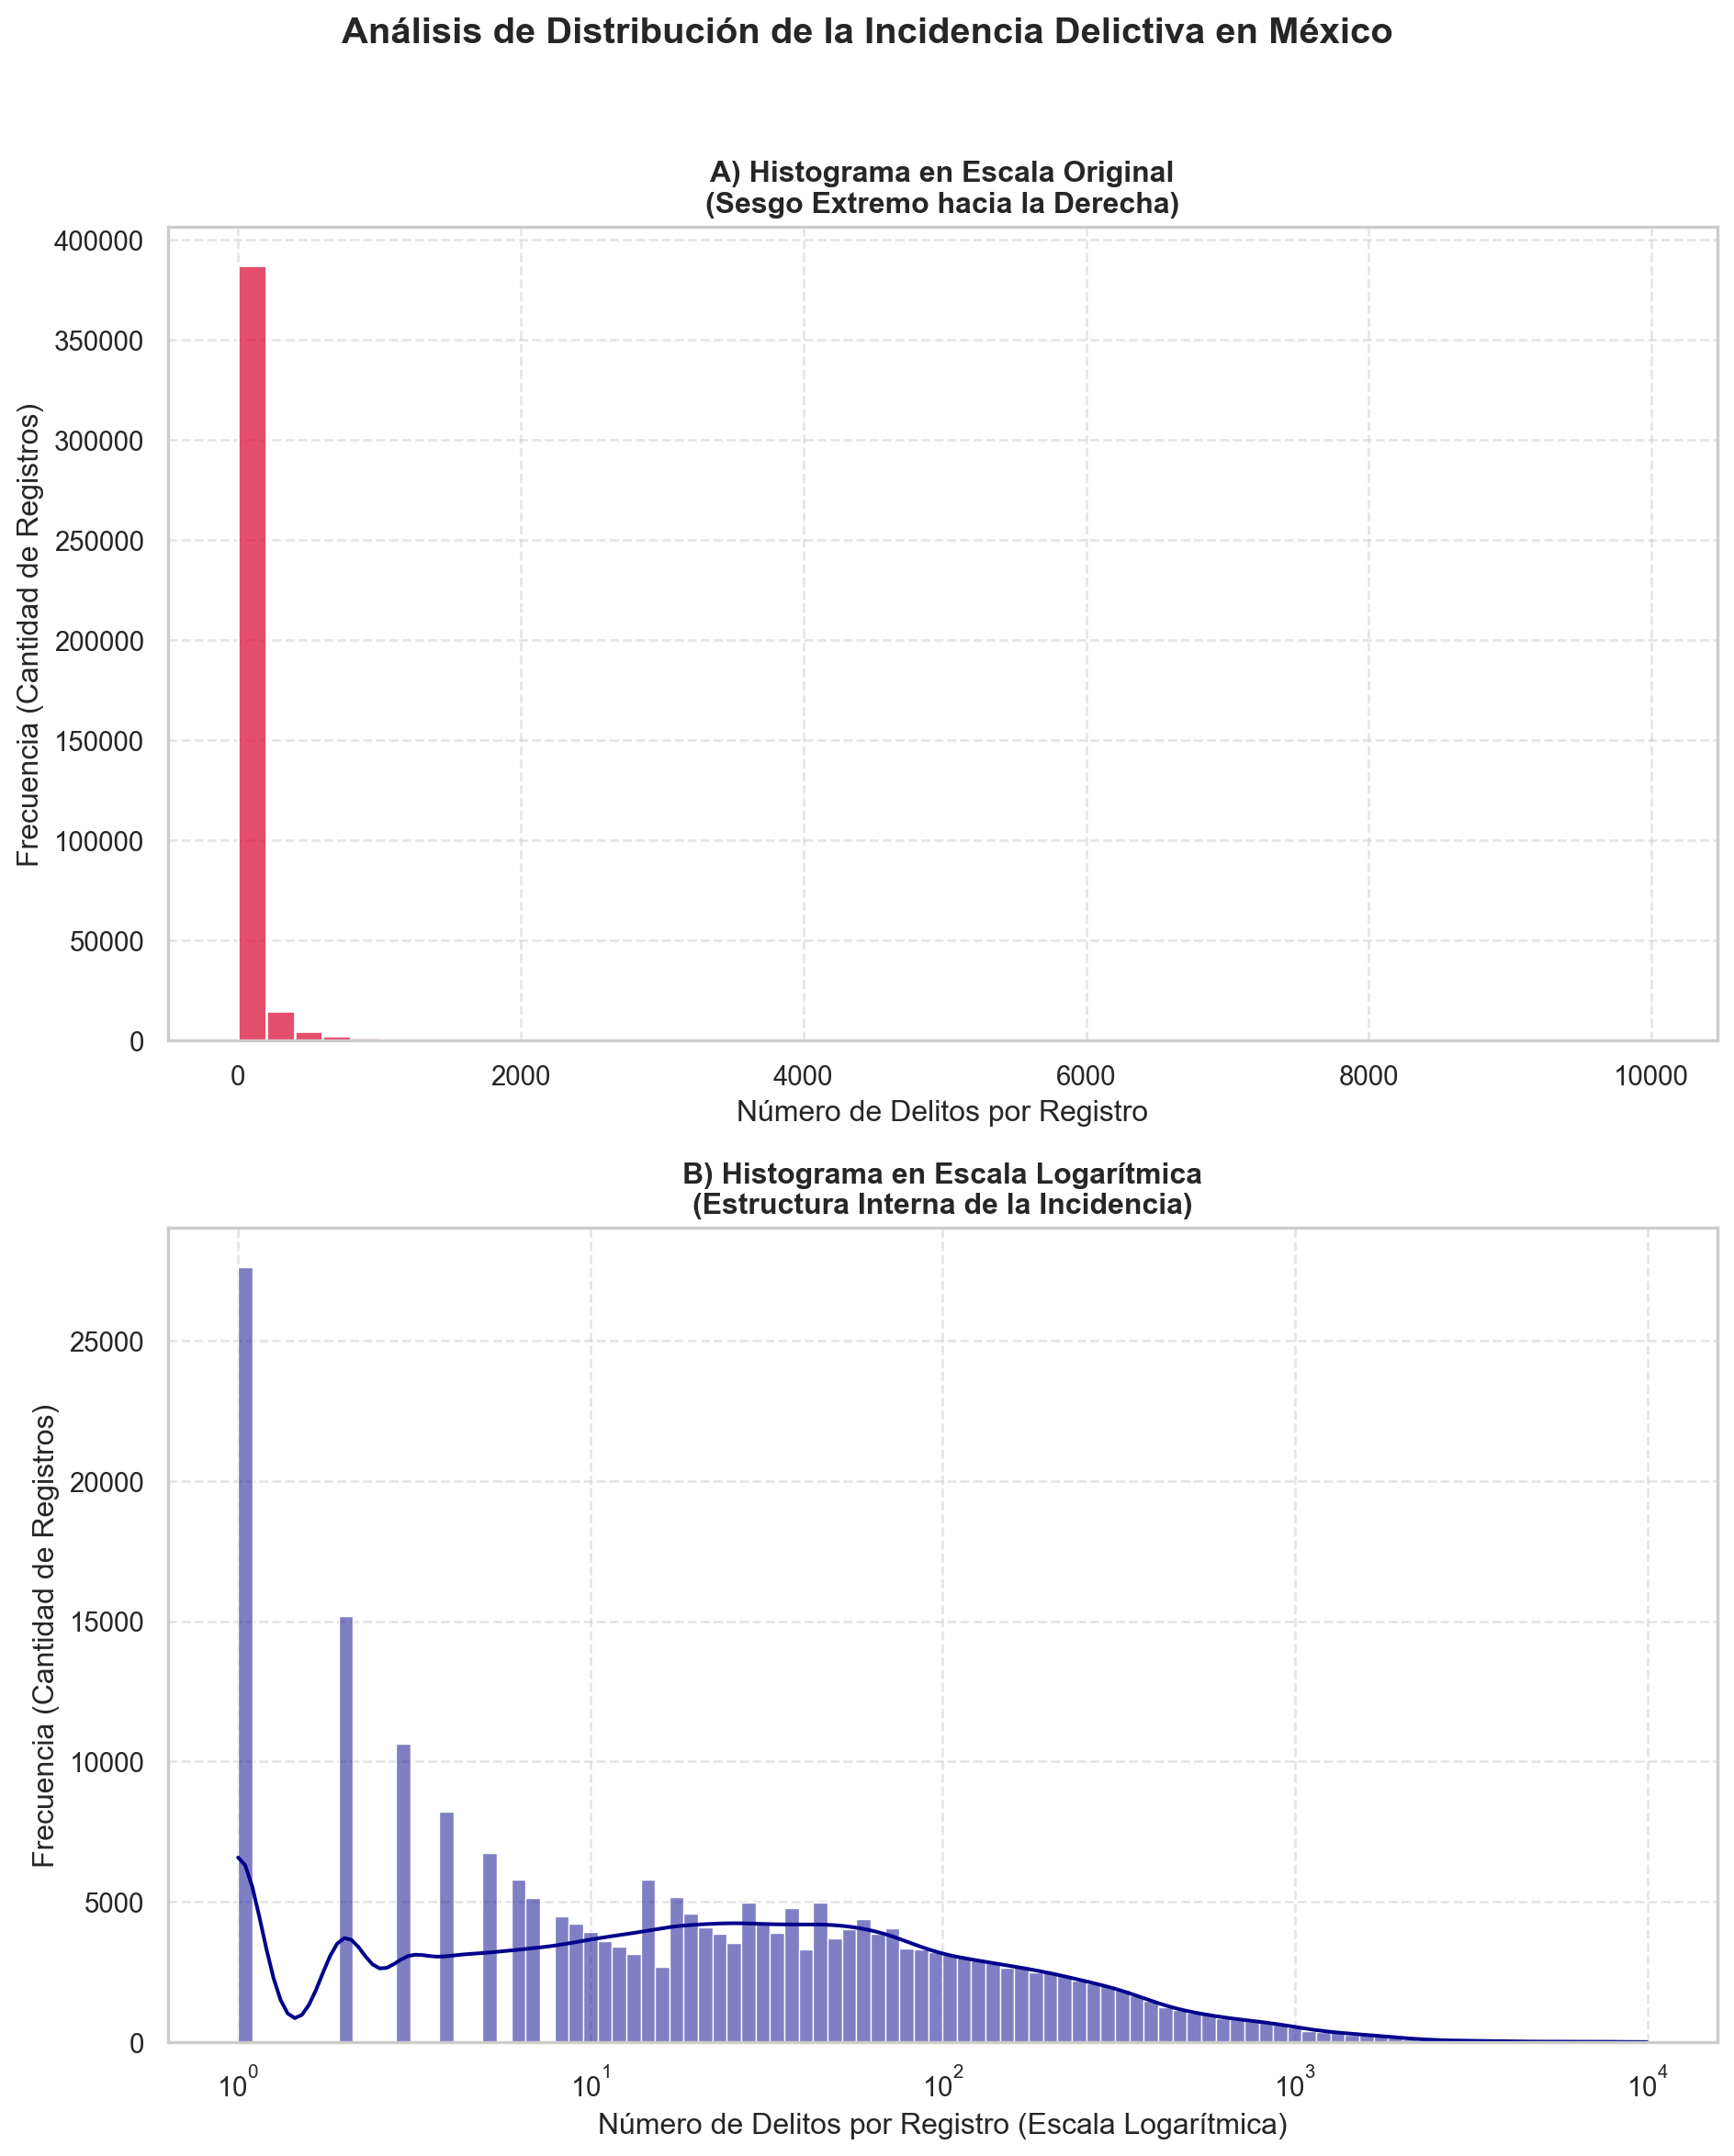
\includegraphics[width=0.75\textwidth]{imagenes/delective-incidence-histograms-output-1.png}
  \caption{Histogramas de Incidencia Delictiva por Estado (marcador de posición)}
  \label{fig:incidence-histograms}
\end{figure}

El primer gráfico muestra una distribución con un sesgo hacia la derecha extremadamente severa. La inmensa mayoría de los registros
del dataset se concentran de forma masiva en valores muy cercanos a cero (recordemos que la mediana del dataset es de 2 delitos por registro).
Esto se debe a que existen muchas categorías de delitos poco comunes o entidades con menor población que reportan frecuentemente cero u
muy pocas incidencias mensuales de estos delitos no tan comúnes. Visualmente, esto genera una gran "pared" en el extremo izquierdo
y una cola invisible infinitamente larga hacia la derecha que se extiende hasta el valor máximo de 9,968.

Con el segundo gráfico queremos reevelar la distribución real que queda oculta bajo el sesgo. Para esto se aplicó una escala logarítmica
sobre el eje de las abscisas (filtrando los registros con elitos). Esto nos da distribución con dos picos:

\begin{itemize}
  \item El primero muestra cuando se registran de 1 a 3 delitos en promedio. Esto representa la gran masa de reportes delictivos de baja
ocurrencia o zonas con baja densidad demográfica.
  \item El segundo muestra cuando se registran de 30 a 100 delitos en promedio. Esto representa la acumulación de delitos altamente recurrentes
(como variantes de robos) en zonas urbanas o de alta incidencia.
\end{itemize}

\subsection{Estadísticas Descriptivas Categóricas}

\begin{lstlisting}[language=Python, caption={Código para obtener estadísticas descriptivas categóricas}, label={lst:stats-descriptivas-categoricas}]
	stats.categorical_stats()
\end{lstlisting}

\begin{table}[ht]
  \centering
  \caption{Estadísticas Descriptivas Categóricas}
  \scriptsize
  \resizebox{\textwidth}{!}{%
    \begin{tabular}{r r r l p{3.5cm} p{3cm} p{3cm} p{2.5cm} l l r l}
      \hline
      \textbf{idx} & \textbf{columna} & \textbf{valores únicos} & \textbf{moda} & \textbf{frecuencia modal} \\
      0 & fecha & 132 & 2015-04-01 & 3136 \\
      1 & entidad & 32 & Aguascalientes & 12936 \\
      2 & bien\_juridico\_afectado & 7 & El patrimonio & 177408 \\
      3 & tipo\_delito & 40 & Robo & 152064 \\
      4 & subtipo\_delito & 55 & Robo de maquinaria & 25344 \\
      5 & modalidad & 59 & Con violencia & 50688 \\
      \hline
    \end{tabular}%
  }
  \label{tab:categorical-stats}
\end{table}

En cuanto a las variables categóricas del conjunto de datos podemos notar hechos bastante interesantes a pesar de la inmensidad del dataset:

\begin{itemize}
  \item El dataset es de 11 años, sin embargo, solo hay 132 fechas únicas, con la fecha inicial siendo el 01 de enero de 2015
  \item La moda del dataset tiene algunos resultados curiosos. Este conjunto de datos es simetrico para cada estado, ya que existen 12936
líneas para c/u. Entonces, al querer cálcular la moda se toma el valor inicial de manera alfabética y resulta ser Aguascalientes.
Sin embargo, esto no significa que sea la entidad con mayor apariciones del dataset.
  \item Lo anterior pasa de igual manera con la fecha, ya que toma la primera fecha del dataset para calcular este valor.
  \item El dataset reporta 40 tipos de delitos únicos reportados, con Robo siendo la categoría principal.
\end{itemize}

Veamos ahora un análisis más detallado de las variables categóricas.

\subsubsection{Delitos más Comunes}

\begin{lstlisting}[language=Python, caption={Código para generar gráfico de los delitos más comunes}, label={lst:delitos-mas-comunes}]
crime_counts = dataframe["tipo_delito"].value_counts().head(10)

fig, ax = plt.subplots(figsize=(10, 4))
crime_counts.plot(kind="barh", ax=ax, color="steelblue")
ax.set_title("Top 10 Tipos de Delito", fontsize=13, fontweight="bold")
ax.set_xlabel("Número de Registros")
ax.invert_yaxis()

# Añade valores en las barras
for i, v in enumerate(crime_counts.values):
    ax.text(v + 1000, i, f"{v:,}", va="center", fontsize=10)

plt.tight_layout()
plt.show()
\end{lstlisting}

\begin{figure}[H]
  \centering
  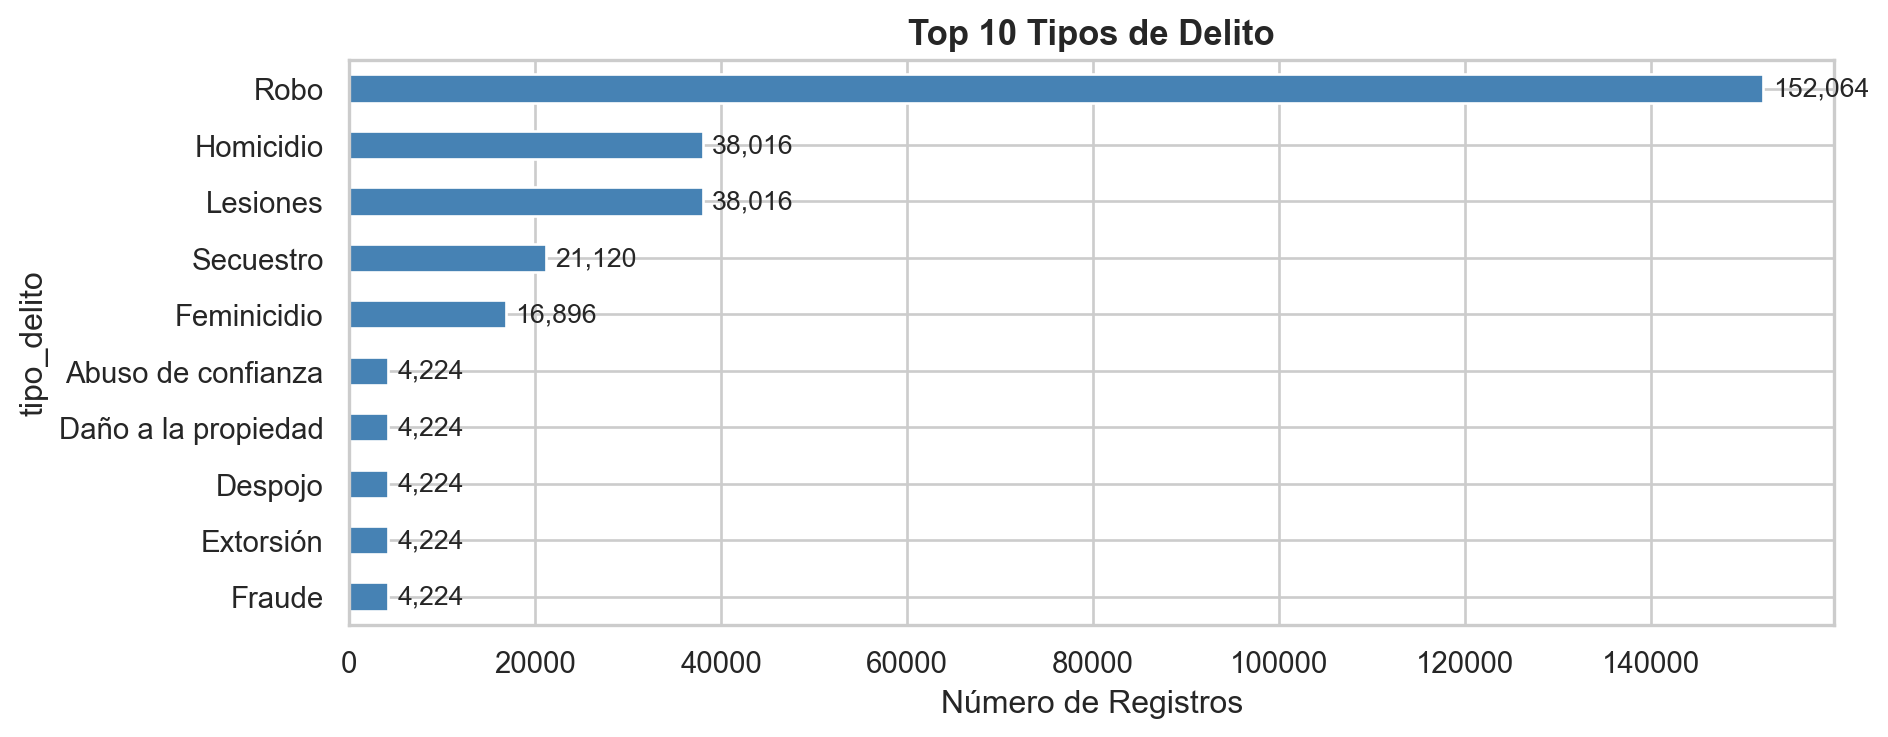
\includegraphics[width=0.85\textwidth]{imagenes/most-common-crimes-output-1.png}
  \caption{Top 10 Tipos de Delito}
  \label{fig:top-crimes}
\end{figure}

Como se mencionaba en la tabla anterior, robo es el delito más reportado, seguido de homicidio y lesiones. Algo a recordar
es que aunque los feminicidios son también homicidios éstos están en una categoriá separada debido al motivo por el que ocurren.
Vemos también que hay una extraña coincidencia de valores entre Abuso de Confianza, Daño a la Propiedad, Despojo, Extorsión y Fraude,
lo que sugiere un sesgo al momento de reportar estos delitos por parte de la autoridad (por ejemplo, cifras redondeadas, reportes nulos, etc.)

\subsubsection{Incidencia Delictiva por Estado}

\begin{lstlisting}[language=Python, caption={Código para generar gráfico de incidencia delictiva por estado}, label={lst:incidencia-delictiva-por-estado}]
from matplotlib.ticker import StrMethodFormatter

entidad_counts = (
    dataframe.groupby("entidad")["incidencia_delictiva"]
    .sum()
    .sort_values(ascending=False)
    .head(10)
)

fig, ax = plt.subplots(figsize=(10, 6))
bars = ax.bar(entidad_counts.index, entidad_counts.values, color="coral")
# Formato del eje Y con separadores de miles y sin decimales
ax.yaxis.set_major_formatter(StrMethodFormatter("{x:,.0f}"))
# Agregamos los valores reales arriba de cada barra con separadores de miles
ax.bar_label(bars, fmt="{:,.0f}", padding=3, fontsize=10, fontweight="bold")

ax.set_title(
    "Incidencia Delictiva Total por Entidad (Top 10) - 2015 a 2025",
    fontsize=15,
    fontweight="bold",
    pad=15,
)
ax.set_ylabel("Total de Delitos", fontsize=12)
ax.set_xlabel("Entidad Federativa", fontsize=12)
ax.tick_params(axis="x", rotation=40)

plt.tight_layout()
plt.show()
\end{lstlisting}

\begin{figure}[H]
  \centering
  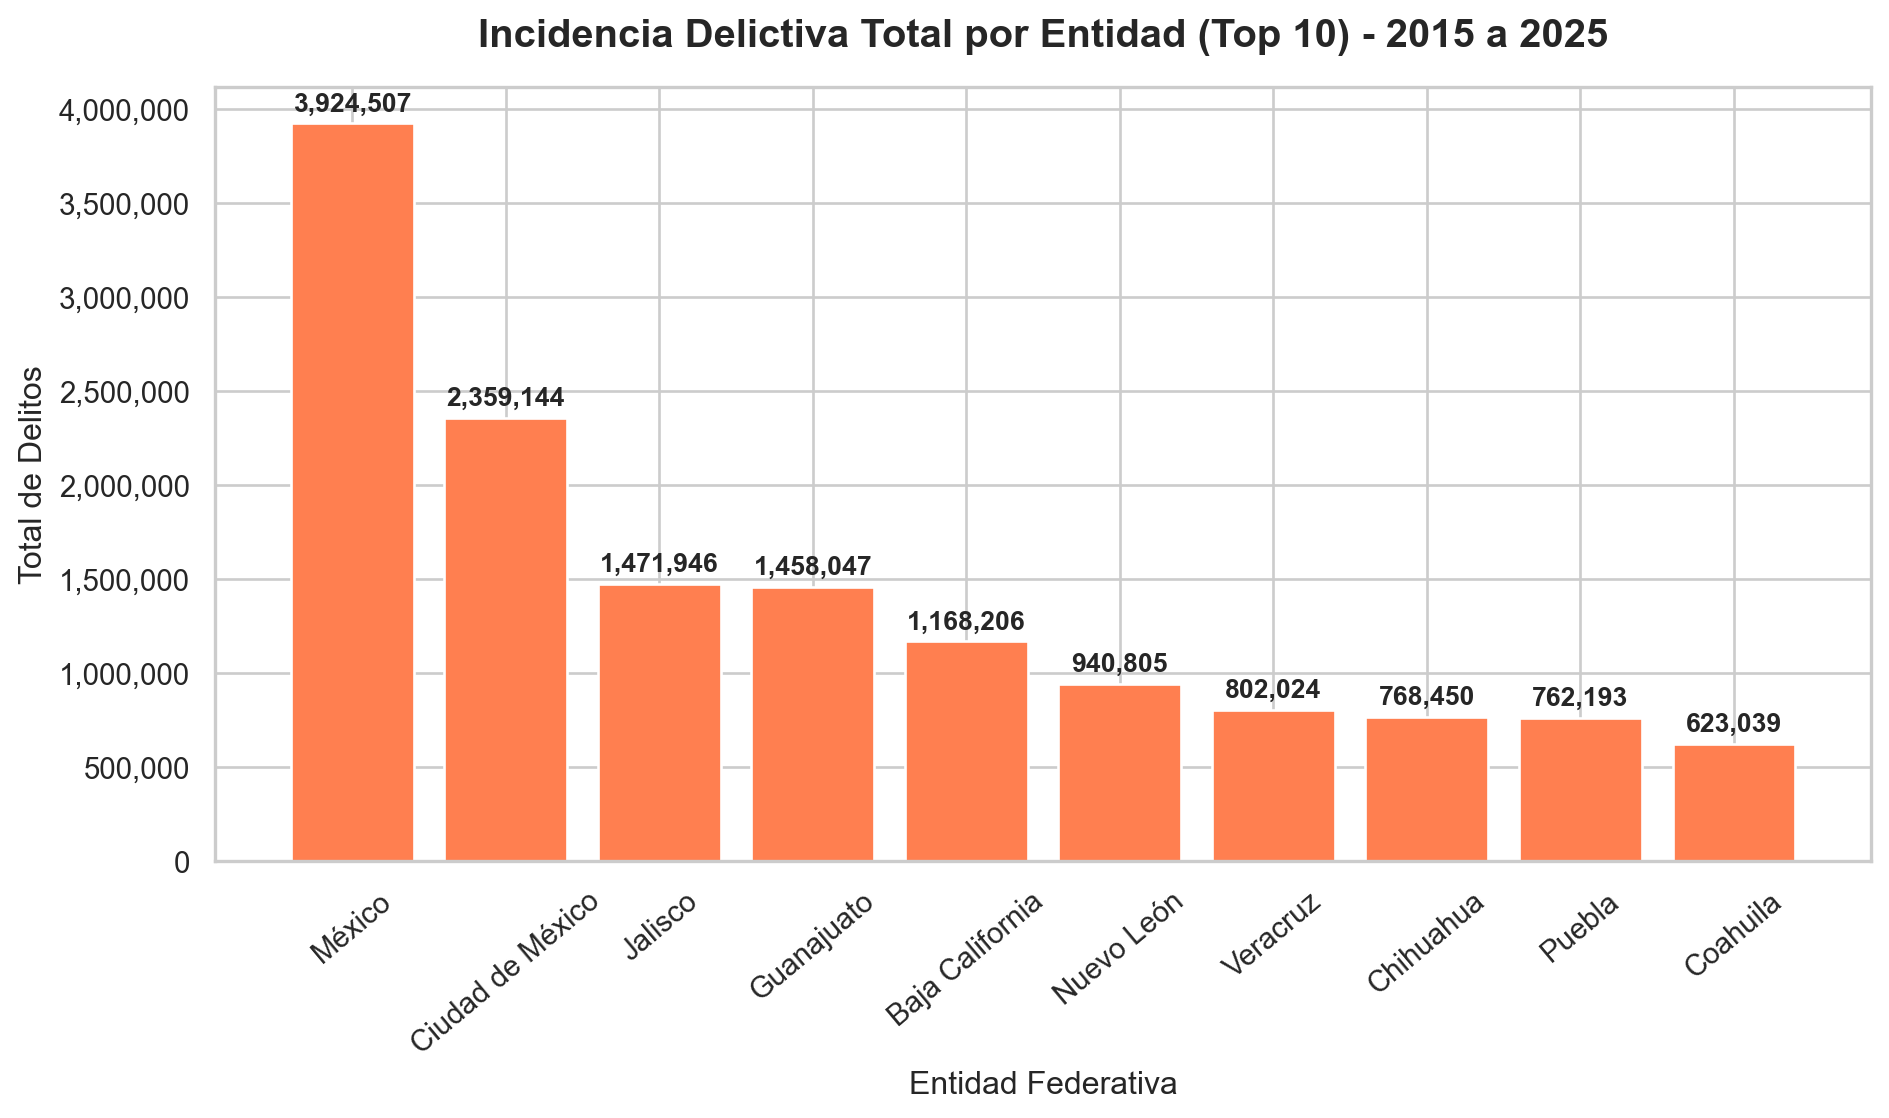
\includegraphics[width=0.8\textwidth]{imagenes/crime-by-state-output-1.png}
  \caption{Incidencia Delictiva Total por Entidad}
  \label{fig:crime-by-state}
\end{figure}

Nuestra sospecha anterior que la EdoMex y la CDMX son los estados con más reportes es correcta. Vemos que le siguen Jalisco,
Guanajuato y Baja California y que, a pesar de la moda, Aguascalientes no figura dentro de los estados con más delitos reportados.

\begin{lstlisting}[language=Python, caption={Código para generar mapa de calor de incidencia por entidad y tipo de delito}, label={lst:heatmap-incidencia-por-entidad-y-delito}]
top_crimes = dataframe["tipo_delito"].value_counts().head(10).index
top_entities = dataframe["entidad"].value_counts().head(10).index

filtered_df = dataframe[dataframe["tipo_delito"].isin(top_crimes) & dataframe["entidad"].isin(top_entities)]

pivot = filtered_df.pivot_table(
    values="incidencia_delictiva", index="entidad", columns="tipo_delito", aggfunc="sum"
)

fig, ax = plt.subplots(figsize=(10, 10))
sns.heatmap(
    pivot,
    cmap="RdYlGn_r",
    annot=True,
    fmt=",.0f",  # Agregamos la coma para que los números dentro del mapa tengan comas (ej. 1,234,567)
    cbar_kws={"label": "Incidencia"},
    ax=ax,
)

cbar = ax.collections[0].colorbar
# aplicamos formato con comas de miles y sin decimales
cbar.ax.yaxis.set_major_formatter(StrMethodFormatter('{x:,.0f}'))

ax.set_title(
    "Incidencia por Entidad y Tipo de Delito",
    fontsize=12,
    fontweight="bold",
    pad=15
)

plt.tight_layout()
plt.show()
\end{lstlisting}

\begin{figure}[H]
  \centering
  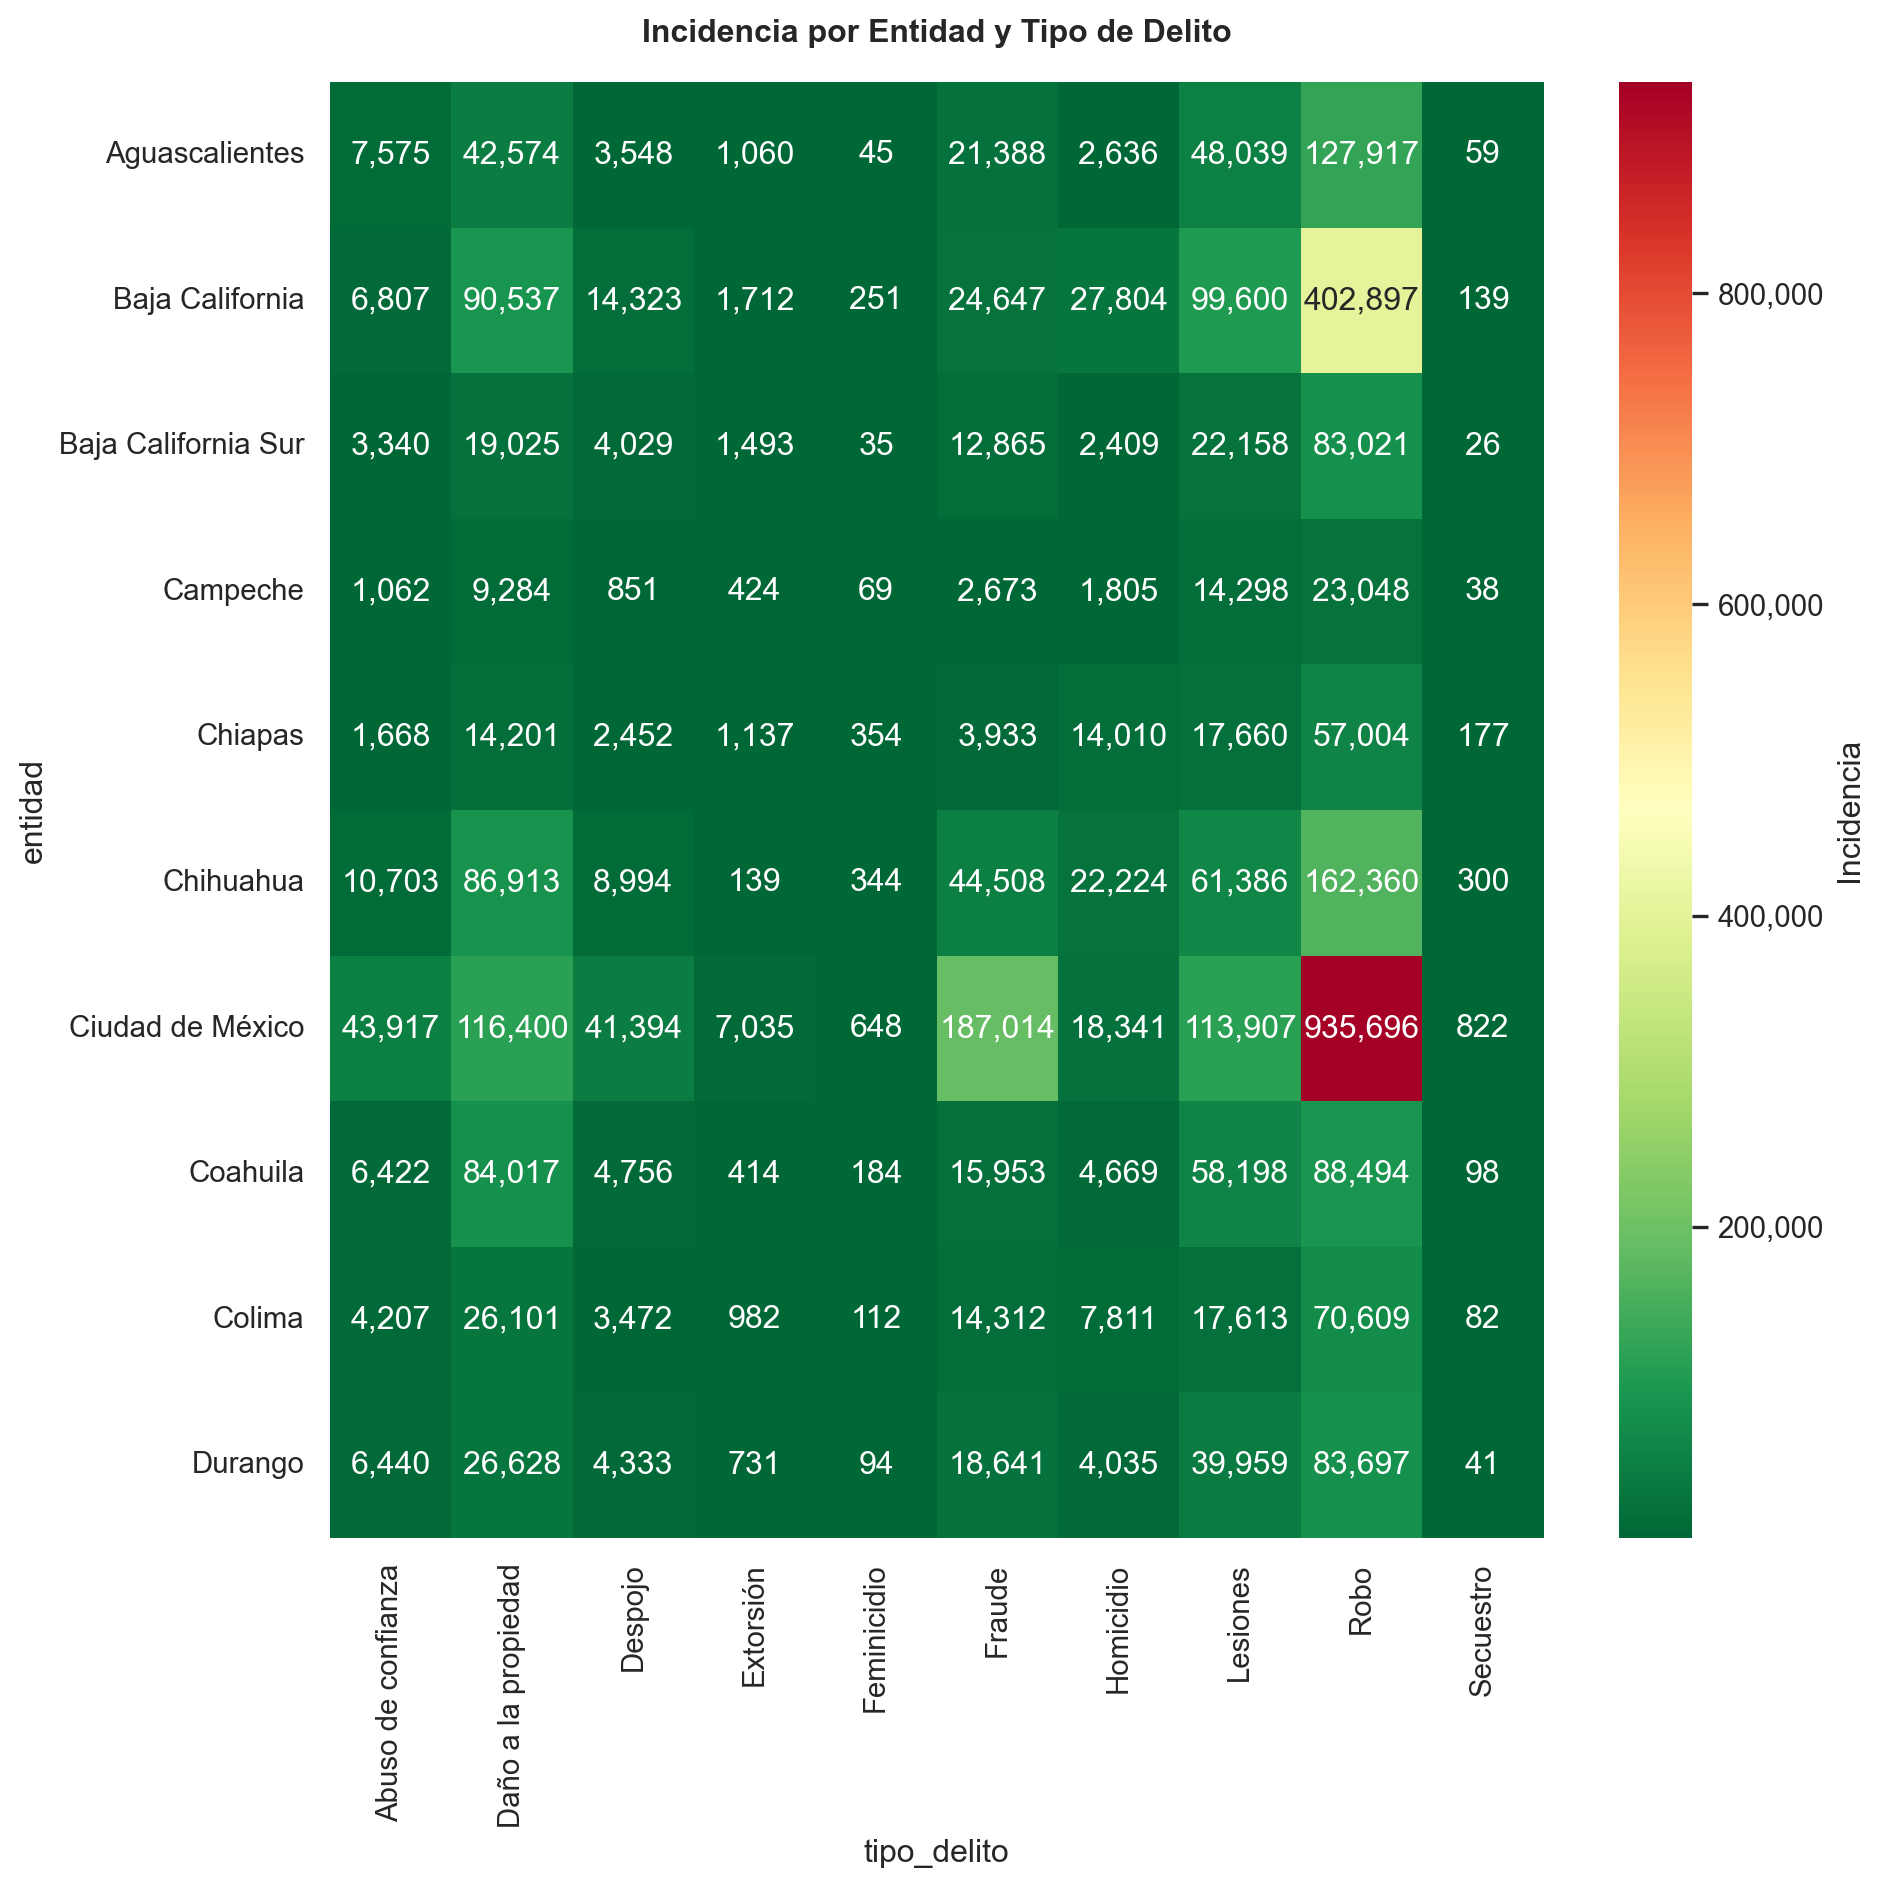
\includegraphics[width=0.8\textwidth]{imagenes/crime-heatmap-output-1.png}
  \caption{Mapa de calor de incidencia por entidad y tipo de delito}
  \label{fig:crime-heatmap}
\end{figure}

\subsubsection{Bienes Jurídicos más Afectados}

\begin{lstlisting}[language=Python, caption={Código para generar gráfico de bienes jurídicos más afectados}, label={lst:bienes-juridicos-mas-afectados}]
bien_juridico = dataframe["bien_juridico_afectado"].value_counts()

fig, ax = plt.subplots(figsize=(8, 8))
wedges, texts, autotexts = ax.pie(
    bien_juridico.values, labels=bien_juridico.index, autopct="%1.1f%%", startangle=90
)
ax.set_title(
    "Distribución de Delitos por Bien Jurídico Afectado", fontsize=11, fontweight="bold"
)
for autotext in autotexts:
    autotext.set_color("white")

plt.show()
\end{lstlisting}

\begin{figure}[H]
	\centering
	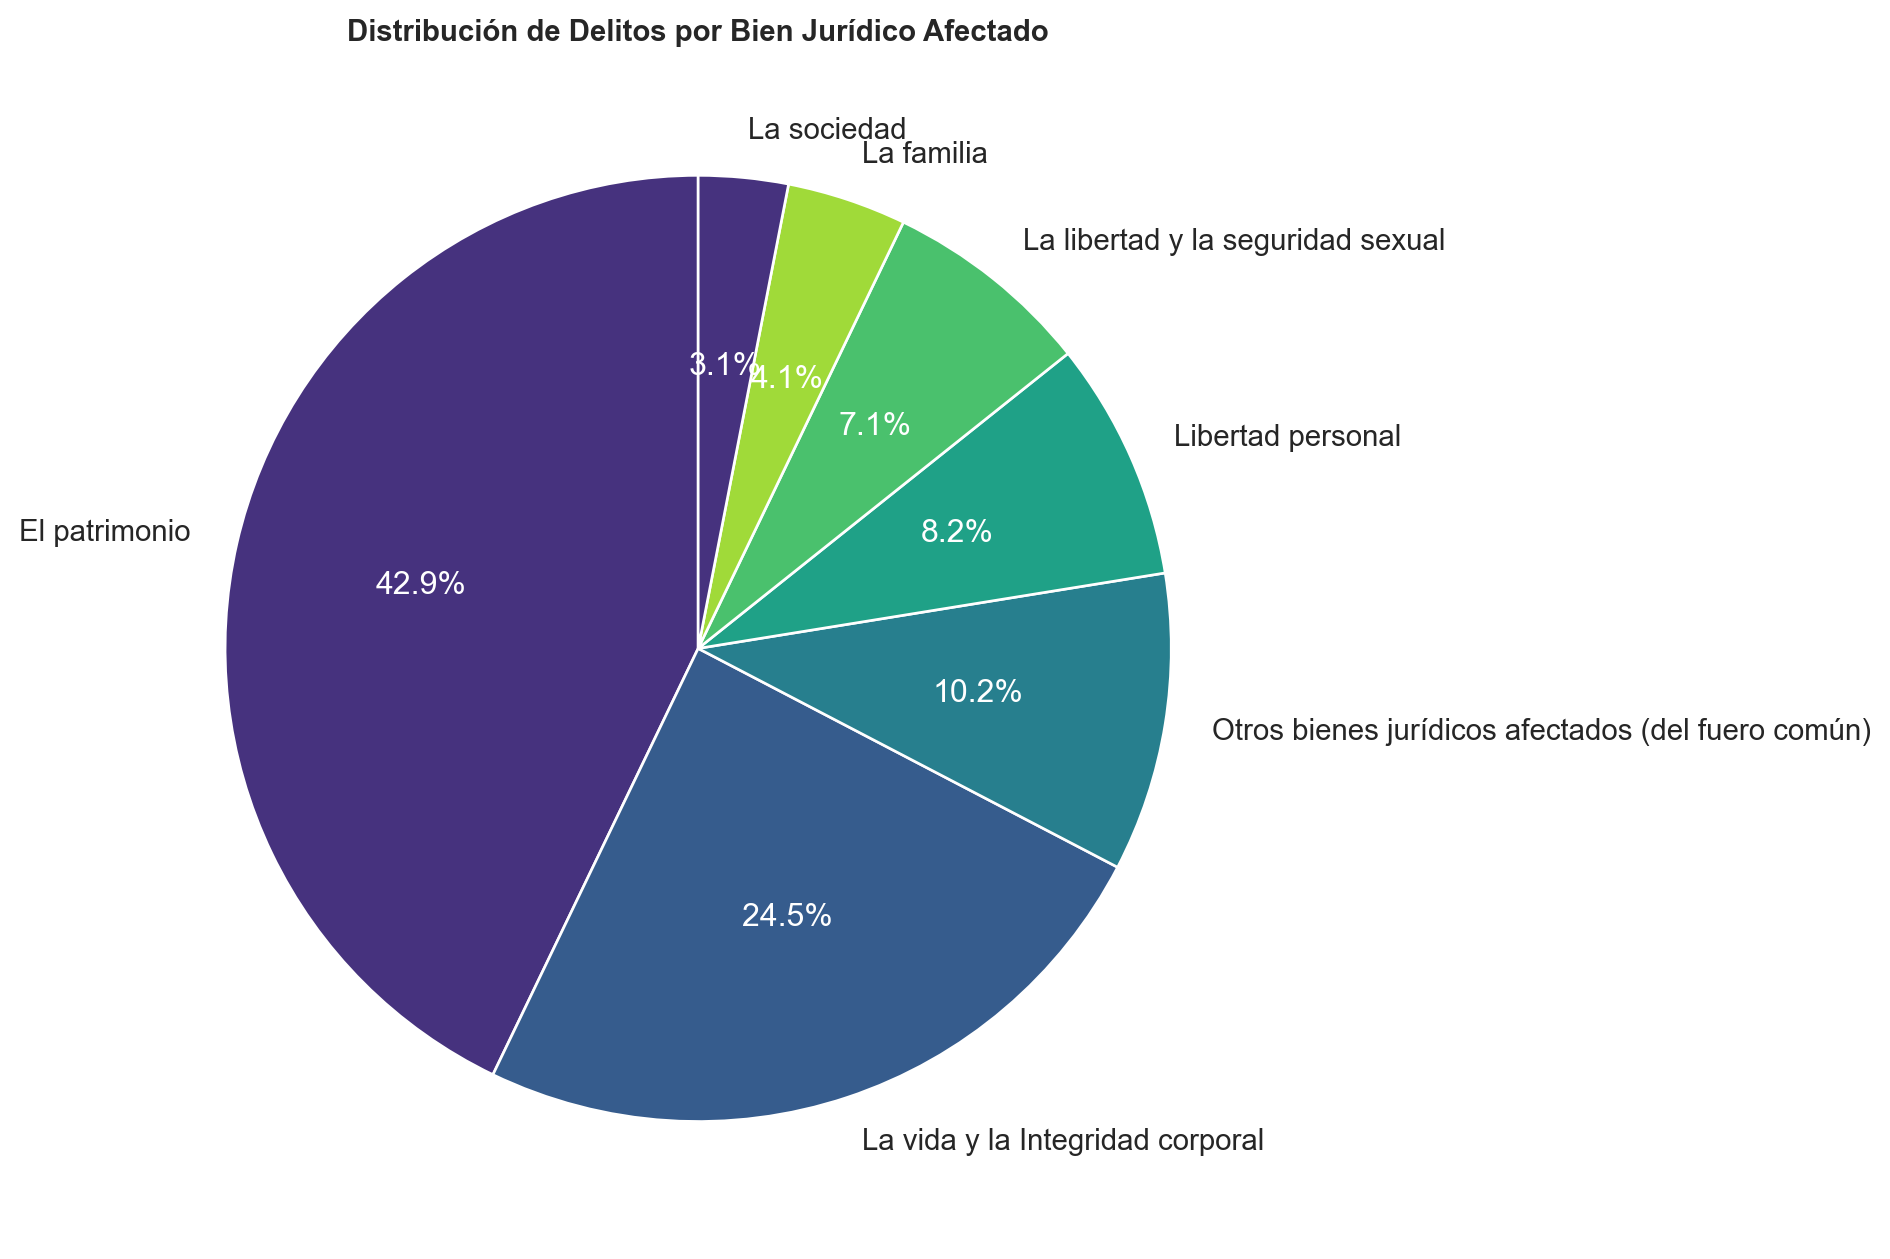
\includegraphics[width=0.75\textwidth]{imagenes/affected-legal-assets-output-1.png}
	\caption{Bienes Jurídicos más Afectados por Delitos en México (2015-2025)}
	\label{fig:affected-legal-assets}
\end{figure}

Para entender esta gráfica debemos entender que la ley define como ‘bienes jurídicos’ a aquellos objetos o relaciones, tangibles o intangibles, que
cuentan con la protección de la ley, como un inmueble, la vida, dinero, etc. En particular, debemos entender que 'El patrimonio' hace referencia al
conjunto de bienes, derechos y obligaciones de una persona, susceptibles de valoración económica. Lo anterior, en otros términos, se refiere a
pertenencias que hemos comprado, dinero que tenga un individuo, etc, pero que tengan relevancia ecónomica.

Ahora pues, tomando en cuenta de que el delito más reportado es el robo, que el patrimonio sea el bien más afectado tiene mucho sentido. Luego, al
ser el homicidio, lesiones, secuestro y feminicidio los delitos que siguen en frecuencia, hace nuevamente sentido que la vida e integridad corportal
sean el segundo bien más afectado.

\subsubsection{Modalidad de los Delitos}

\begin{lstlisting}[language=Python, caption={Código para generar gráfico de modalidades de los delitos}, label={lst:modalidades-delitos}]
modalidad = dataframe["modalidad"].value_counts().head(15)

fig, ax = plt.subplots(figsize=(10, 10))
modalidad.plot(kind="barh", ax=ax, color=["#d62728", "#2ca02c"])

ax.set_title("Distribución de Delitos por Modalidad (Top 10, 2015-2025)", fontsize=10, fontweight="bold")
ax.set_xlabel("Número de Registros")

for i, v in enumerate(modalidad.values):
    ax.text(v + 500, i, f"{v:,}", va="center")

plt.tight_layout()
plt.show()
\end{lstlisting}

\begin{figure}[H]
    \centering
    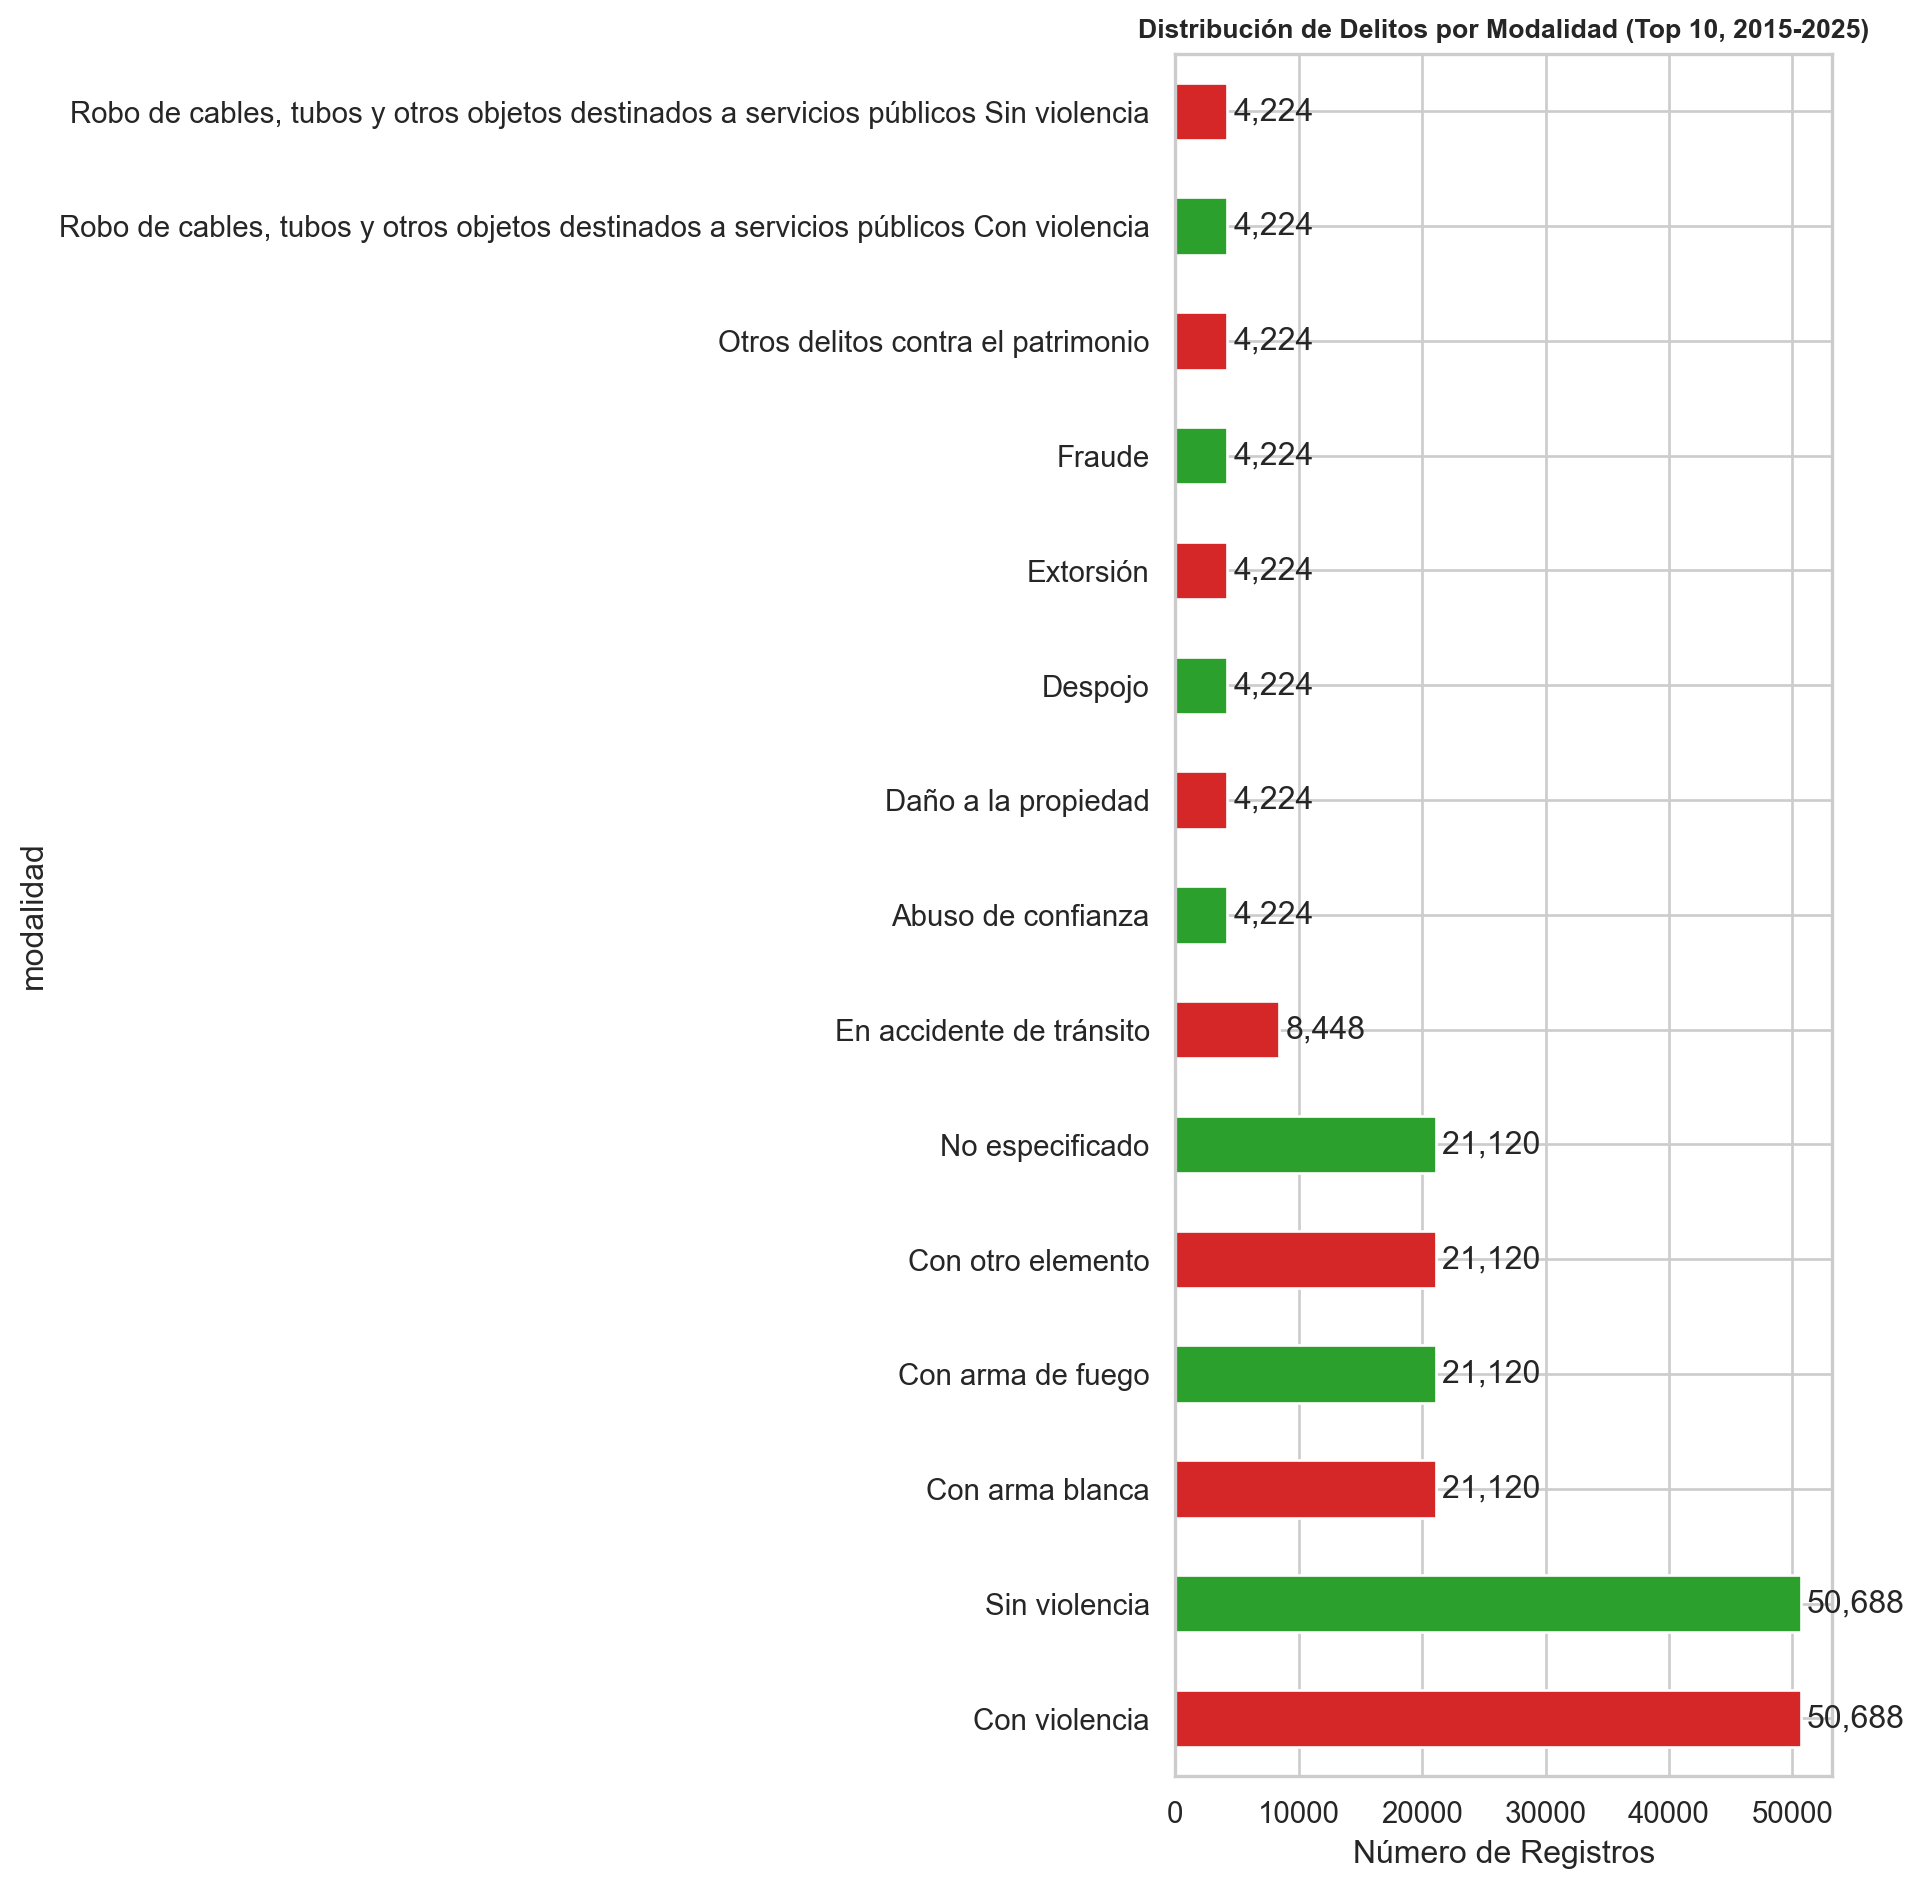
\includegraphics[width=0.7\textwidth]{imagenes/crime-modality-output-1.png}
    \caption{Modalidad de los Delitos en México (2015-2025)}
    \label{fig:crime-modalities}
\end{figure}

Nuevamente, vemos también que hay una extranña coincidencia de valores después de la modalidad ‘En Accidente
de Tráfico’, lo que sugiere y mantiene la idea de que existe un gran sesgo al momento de reportar correctamente
todos los delitos.

También notamos que no existe una única forma de reportar los delitos con violencia, por lo que un registro
puede pertenecer a un delito con ésta modalidad y ser asignado a otra categoria (sobre todo en lo referente
a los subtipos de robo).

\subsubsection{Delincuencia por Año}

\begin{lstlisting}[language=Python, caption={Código para generar gráfico de delincuencia por año}, label={lst:delincuencia-por-año}]
dataframe["fecha"] = pd.to_datetime(dataframe["fecha"])  # add this line before groupby
temporal = dataframe.groupby("fecha")["incidencia_delictiva"].sum().sort_index()

fig, ax = plt.subplots(figsize=(10, 6))
ax.plot(temporal.index, temporal.values, linewidth=2, color="darkred")
ax.fill_between(temporal.index, temporal.values, alpha=0.2, color="red")

ax.set_title(
    "Evolución Temporal de la Incidencia Delictiva (2015-2025)",
    fontsize=13,
    fontweight="bold",
)
ax.set_xlabel("Fecha")
ax.set_ylabel("Incidencia Delictiva Total")
ax.grid(True, alpha=0.2)
ax.xaxis.set_major_locator(mdates.YearLocator())
ax.xaxis.set_major_formatter(mdates.DateFormatter("%Y"))
ax.xaxis.set_minor_locator(mdates.MonthLocator())
ax.grid(True, which="major", alpha=0.3)
ax.grid(True, which="minor", alpha=0.1)
plt.tight_layout()
plt.show()
```
\end{lstlisting}

\begin{figure}[H]
    \centering
    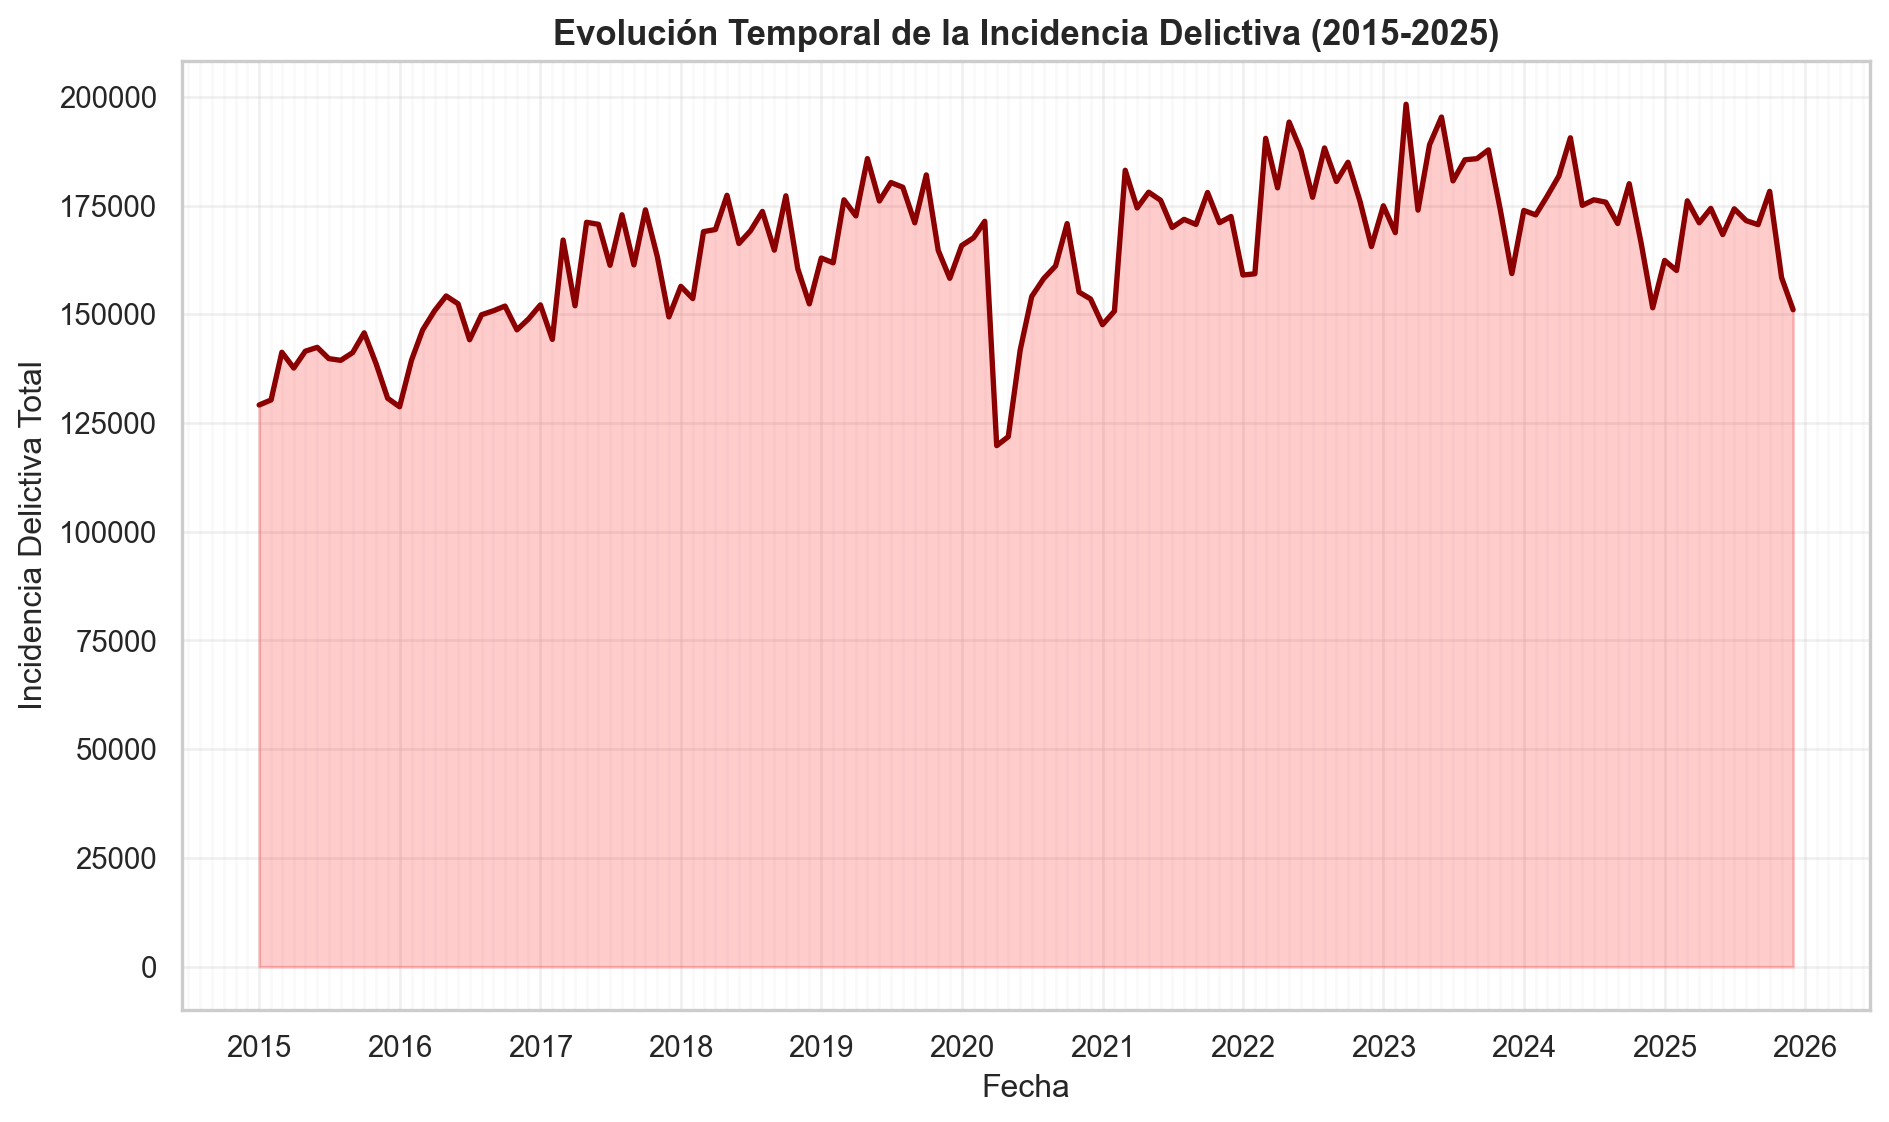
\includegraphics[width=0.8\textwidth]{imagenes/crime-by-year-output-1.png}
    \caption{Evolución Temporal de la Incidencia Delictiva en México (2015-2025)}
    \label{fig:crime-over-time}
\end{figure}

Vemos que, desafortunadamente, no existe un decrecimiento notable en cuanto a la delicuencia en este periodo de tiempo. E incluso, desde 2022
hacia adelante es donde se alcanzan números más alto.

Veamos ahora como se ve ésta evolución dados los meses del año:

\begin{lstlisting}[language=Python, caption={Código para generar gráfico de delincuencia por mes}, label={lst:delincuencia-por-mes}]
dataframe["fecha"] = pd.to_datetime(dataframe["fecha"])
dataframe["año"] = dataframe["fecha"].dt.year
dataframe["mes"] = dataframe["fecha"].dt.month

pivot_data = dataframe.groupby(["año", "mes"])["incidencia_delictiva"].sum().unstack()

fig, ax = plt.subplots(figsize=(10, 10))
sns.heatmap(
    pivot_data,
    cmap="YlOrRd",
    annot=False,
    fmt="d",
    cbar_kws={"label": "Incidencia Delictiva"},
    ax=ax,
)

ax.set_title(
    "Patrón Mensual de Delincuencia por Año (2015-2025)", fontsize=13, fontweight="bold"
)
ax.set_xlabel("Mes")
ax.set_ylabel("Año")

plt.tight_layout()
plt.show()
\end{lstlisting}

\begin{figure}[H]
    \centering
    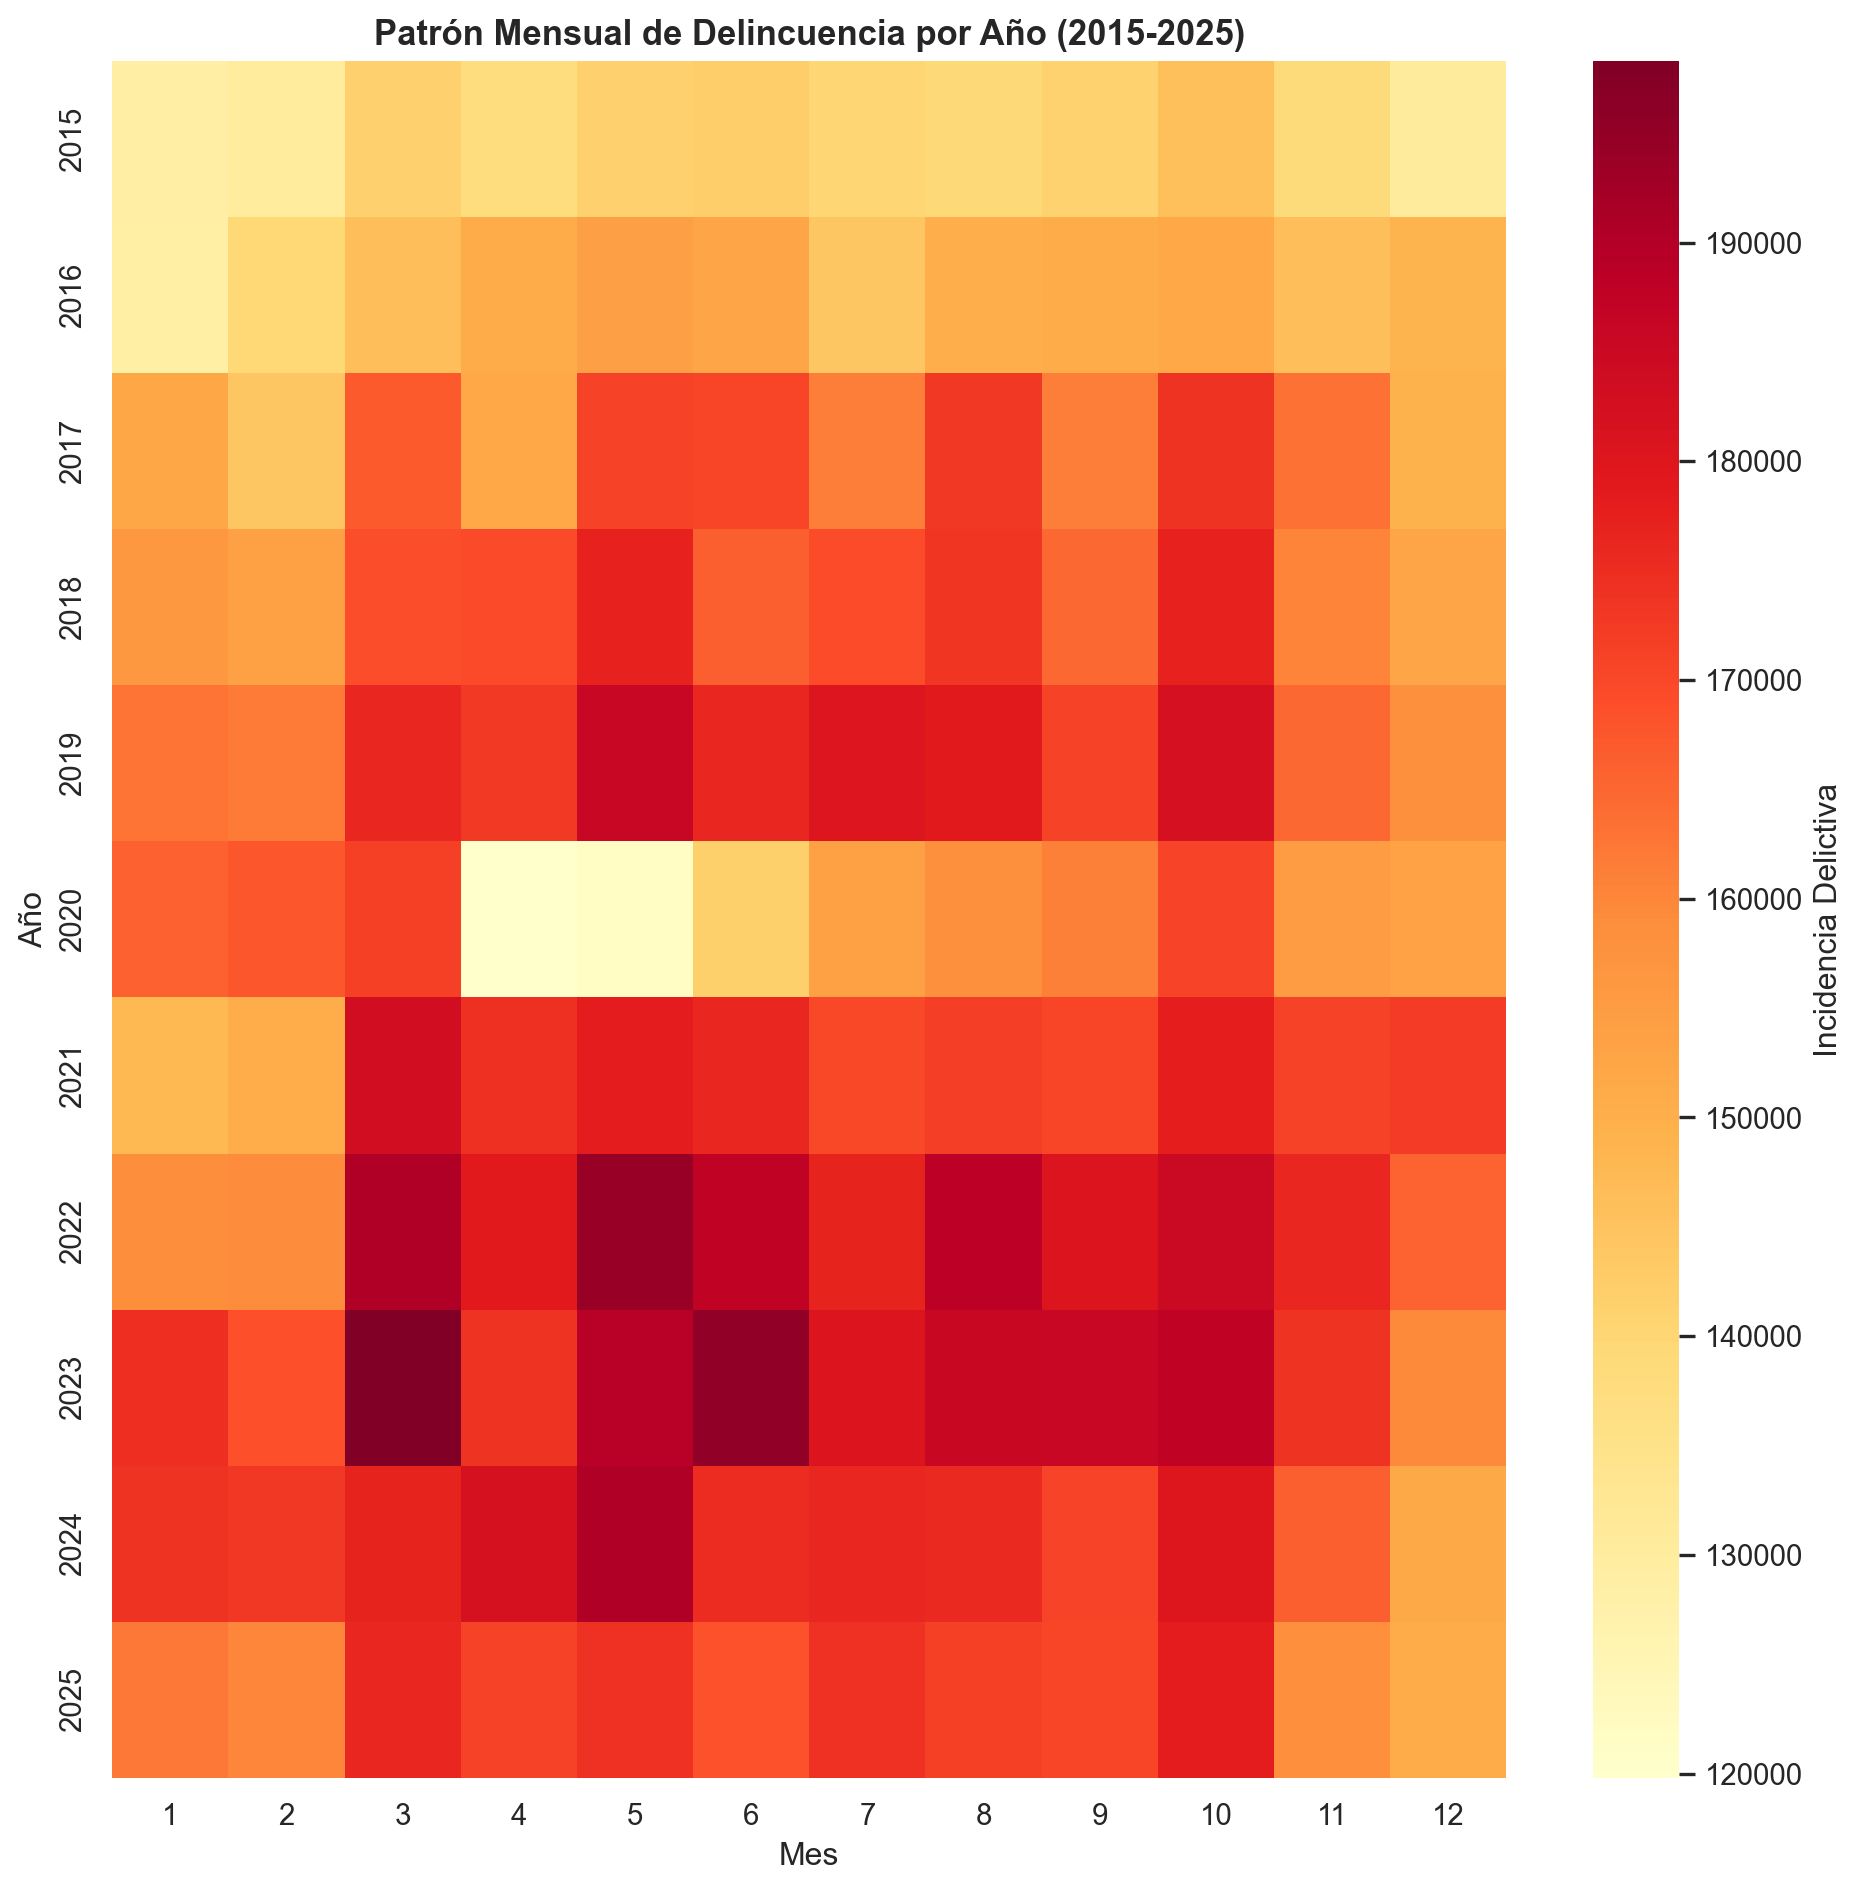
\includegraphics[width=0.8\textwidth]{imagenes/crime-by-month-output-1.png}
    \caption{Patrón Mensual de Delincuencia por Año en México (2015-2025)}
    \label{fig:crime-by-month}
\end{figure}

Vemos que en particular, de 2021 a 2025 el foco ha sido entre Marzo a Junio. Mientras que en años anteriores
habia sido de Mayo a Agosto (2015-2019). Lo que si es más fácil de notar con esto es que 2020 tiene los
valores más bajos de todos los años del conjunto, lo que puede deberse a que la incidencia delicitiva
realmente bajó durante ese periodo o que directamente no se reportó por completo.

\subsection{Detección de Outliers}

Para detectar outliers lo que haremos será ocupar IQR. Por lo anterior notamos que la incidencia delictiva
está fuertemente sesgada a la derecha por la CDMX y Edomex, ya que disparan los valores frente a estados
pequeños. El z-score asume normalidad y los propios extremos inflan media y desviación, así que ocupar ésta
medida reportaría resultados sesgados.

Para esto lo que haremos será ocupar la clase \texttt{OutlierDetector} que, como su nombre lo indica,
identificará los valores atípicos y luego usaremos su método flag() para aplicar ésta identificación a
un nuevo dataframe.

\begin{lstlisting}[language=Python, caption={Código para detectar outliers en la incidencia delictiva}, label={lst:outlier-detection}]
det = OutlierDetector(dataframe, columns=["incidencia_delictiva"])
det.summary()
\end{lstlisting}

\begin{table}[ht]
  \centering
  \caption{Resumen de Detección de Outliers}
  \scriptsize
  \resizebox{\textwidth}{!}{%
    \begin{tabular}{r r r l p{3.5cm} p{3cm} p{3cm} p{2.5cm} l l r l}
      \hline
      \textbf{idx} & \textbf{columna} & \textbf{Q1} & \textbf{Q3} & \textbf{IQR} & \textbf{Límite Inferior} & \textbf{Límite Superior} & \textbf{Número de Outliers} & \textbf{\% de Outliers} \\
      0 & incidencia\_delictiva & 413952 & 0.0 & 9968.0 & -39.0 & 65.0 & 63128 & 15.250077 \\
      \hline
    \end{tabular}%
  }
  \label{tab:outlier-summary}
\end{table}

Vemos que del total de registros, 63128 fueron identificados como outliers, lo que representa aproximadamente el 15.25\% del dataset. Esto es un
porcentaje considerable, pero dado el contexto de la delincuencia en México, es comprensible que existan registros con incidencias extremadamente
altas, especialmente en entidades como la CDMX y el EdoMex.

Sin embargo, es importante destacar que estos outliers no necesariamente representan errores en los datos, sino que reflejan la realidad de la
incidencia delictiva en ciertas regiones y periodos. Por lo tanto, en lugar de eliminar estos registros, se ha optado por marcarlos con una nueva
columna para su posterior análisis y consideración en cualquier modelado o interpretación de los datos. De esta manera, los datos se muestran como
sigue:

\begin{lstlisting}[language=Python, caption={Código para mostrar el dataset con la columna de outliers}, label={lst:dataset-con-outliers}]
det.flag()
\end{lstlisting}

\begin{table}[ht]
  \centering
  \caption{Muestra del dataset con columna de outliers}
  \scriptsize
  \resizebox{\textwidth}{!}{%
    \begin{tabular}{r r r l p{3.5cm} p{3cm} p{3cm} p{2.5cm} l l r l r}
      \hline
      \textbf{id} & \textbf{fecha} & \textbf{entidad} & \textbf{bien\_juridico\_afectado} & \textbf{tipo\_delito} & \textbf{subtipo\_delito} & \textbf{modalidad} & \textbf{incidencia\_delictiva} & \textbf{incidencia\_delectiva\_is\_outlier} \\
      \hline
      0 & 2015-04-01 & Aguascalientes & El patrimonio & Abuso de confianza & Abuso de confianza & Abuso de confianza & 22 & False \\
    1 & 2015-08-01 & Aguascalientes & El patrimonio & Abuso de confianza & Abuso de confianza & Abuso de confianza & 40 & False \\
    2 & 2015-12-01 & Aguascalientes & El patrimonio & Abuso de confianza & Abuso de confianza & Abuso de confianza & 26 & False \\
    3 & 2015-01-01 & Aguascalientes & El patrimonio & Abuso de confianza & Abuso de confianza & Abuso de confianza & 41 & False \\
    4 & 2015-02-01 & Aguascalientes & El patrimonio & Abuso de confianza & Abuso de confianza & Abuso de confianza & 33 & False \\
    \hline
    \end{tabular}%
  }
  \label{tab:dataset-outliers}
\end{table}
    \section{Modelos}

Ahora, lo que buscamos es construir un modelo de regresión capaz de predecir la incidencia delictiva mensual
a nivel estatal en México, utilizando como variables predictoras la entidad federativa, el bien jurídico
afectado, el tipo y subtipo de delito, la modalidad y \emph{features} temporales (año, mes, trimestre).

Para esto utilizaremos un \textbf{Random Forest Regressor} dentro de un pipeline de scikit-learn que incluye lo
siguiente:

\begin{itemize}
  \item \textbf{Preprocesamiento}: codificación One-Hot de variables categóricas y estandarización de variables
  numéricas.
  \item \textbf{Búsqueda de hiperparámetros}: Usaremos \texttt{RandomizedSearchCV} con validación cruzada de 3 pliegues,
  más eficiente que una búsqueda exhaustiva para este volumen de datos.
  \item \textbf{Transformación del objetivo}: Aplicaremos \texttt{log1p} a la variable objetivo para mitigar el sesgo
  observado en el EDA.
\end{itemize}

El dataset contiene $\sim$414,000 registros de incidencia delictiva estatal, por lo que trabajar con todos
estos registros es demasiado pesado en recursos. Es por esto que para este modelo trabajaremos con una
muestra estratificada de 50,000 registros que preserva la proporción de tipos de delito.

El cuaderno de Jupyter Notebook que acompaña esta sección se encuentra disponible haciendo click
\href{https://github.com/wallsified/proyecto-final-aymdd/blob/main/notebooks/models.ipynb}{aquí}.

\begin{lstlisting}[language=Python, caption={Carga de librerías y módulos del proyecto}, label={lst:carga-modelos}]
import sys
from pathlib import Path

sys.path.insert(0, str(Path.cwd().parent))

import pandas as pd
import numpy as np
import matplotlib.pyplot as plt
import seaborn as sns

from sklearn.model_selection import train_test_split

from src.model.preprocesamiento import (
    cargar_preparar_datos,
    separar_features_target,
    construir_preprocesador,
)
from src.model.entrenamiento import entrenar_random_forest
from src.model.evaluacion import evaluar_modelo, grafica_predicciones, grafica_residuales
from src.model.persistencia import guardar_modelo

pd.set_option("display.max_columns", 20)
pd.set_option("display.width", 140)
\end{lstlisting}

\subsection{Carga y preparación de datos}

Cargamos el dataset limpio resultado del EDA y aplicamos un muestreo estratificado sobre la columna
\texttt{tipo\_delito} para reducir los $\sim$414,000 registros a 50,000. Esto preserva la distribución de tipos de
delito y reduce drásticamente el tiempo de entrenamiento sin comprometer la calidad del modelo, ya que
Random Forest muestra rendimientos decrecientes con volúmenes de datos muy grandes.

Luego, separamos las features de nuestra variable objetivo: \texttt{incidencia\_delictiva}, y aplicamos una
transformación logarítmica con \texttt{log1p} para compensar el fuerte sesgo a la derecha observado en el EDA.

\begin{lstlisting}[language=Python, caption={Carga y muestra estratificada del dataset}, label={lst:carga-datos-modelo}]
RUTA_DATOS = str(Path.cwd().parent / "data" / "processed" / "INM_estatal_dic25_clean.csv")

df = cargar_preparar_datos(RUTA_DATOS)
print(f"Muestra estratificada: {df.shape[0]:,} filas x {df.shape[1]} columnas")
df.head(3)
\end{lstlisting}

\begin{lstlisting}
Muestra estratificada: 50,000 filas x 7 columnas
\end{lstlisting}

\begin{table}[ht]
  \centering
  \caption{Primeras filas del dataset muestreado}
  \resizebox{\textwidth}{!}{%
    \begin{tabular}{l l l l l l l l}
      \hline
      \textbf{idx} & \textbf{fecha} & \textbf{entidad} & \textbf{bien\_juridico\_afectado} & \textbf{tipo\_delito} & \textbf{subtipo\_delito} & \textbf{modalidad} & \textbf{incidencia\_delictiva} \\
      \hline
      249379 & 2021-03-01 & Puebla & El patrimonio & Otros delitos contra el patrimonio & Otros delitos contra el patrimonio & Otros delitos contra el patrimonio & 26 \\
      57395 & 2016-09-01 & Morelos & La vida y la Integridad corporal & Lesiones & Lesiones dolosas & No especificado & 144 \\
      289658 & 2022-12-01 & Quintana Roo & El patrimonio & Robo & Robo de vehículo automotor & Robo de coche de 4 ruedas Con violencia & 11 \\
    \end{tabular}%
  }
  \label{tab:primeras-filas-modelo}
\end{table}

La columna \texttt{fecha}, al ser de tipo datetime, se descompone en tres features numéricas: \texttt{anio}, \texttt{mes} y
\texttt{trimestre}. Esto permite al modelo capturar tendencias temporales (tendencia anual, estacionalidad mensual
y patrones por trimestre) sin introducir alta cardinalidad como haría un One-Hot de fechas individuales.

\begin{lstlisting}[language=Python, caption={Separación de features y target con transformación log1p}, label={lst:features-target}]
X, y = separar_features_target(df)

print(f"Features: {X.shape[1]} columnas")
print(f"Columnas: {list(X.columns)}")
print(f"\nTarget (log1p) - media: {y.mean():.3f}, std: {y.std():.3f}")
X.head(3)
\end{lstlisting}

\begin{lstlisting}
Features: 8 columnas
Columnas: ['entidad', 'bien_juridico_afectado', 'tipo_delito', 'subtipo_delito', 'modalidad', 'anio', 'mes', 'trimestre']

Target (log1p) - media: 1.753, std: 1.990
\end{lstlisting}

\begin{table}[ht]
  \centering
  \caption{Primeras filas de las features (X) y el target transformado (y)}
  \resizebox{\textwidth}{!}{%
    \begin{tabular}{l l l l l l l l l}
      \hline
      \textbf{idx} & \textbf{entidad} & \textbf{bien\_juridico\_afectado} & \textbf{tipo\_delito} & \textbf{subtipo\_delito} & \textbf{modalidad} & \textbf{anio} & \textbf{mes} & \textbf{trimestre} \\
      \hline
      249379 & Puebla & El patrimonio & Otros delitos contra el patrimonio & Otros delitos contra el patrimonio & Otros delitos contra el patrimonio & 2021 & 3 & 1\\
      57395 & Morelos & La vida y la Integridad corporal & Lesiones & Lesiones dolosas & No especificado & 2016 & 9 & 3\\
      289658 & Quintana Roo & El patrimonio & Robo & Robo de vehículo automotor & Robo de coche de 4 ruedas Con violencia & 2022 & 12 & 4 \\
      \hline
    \end{tabular}%
  }
  \label{tab:features-target}
\end{table}


\subsection{Preprocesamiento y división train/test}

Separamos el 80\% de los datos para entrenamiento y el 20\% restante para prueba, con una semilla fija para
reproducibilidad.

El preprocesador aplica dos transformaciones dentro del pipeline:

\begin{itemize}
  \item \textbf{OneHotEncoder} sobre las columnas categóricas (\texttt{entidad}, \texttt{bien\_juridico\_afectado}, \texttt{tipo\_delito},
  \texttt{subtipo\_delito}, \texttt{modalidad}). Esto para convertir cada categoría en una columna binaria. Se configura
  \texttt{handle\_unknown="ignore"} para que no falle si aparece una categoría nueva en el conjunto de prueba.
  \item \textbf{StandardScaler} sobre las columnas numéricas (\texttt{anio}, \texttt{mes}, \texttt{trimestre}) para estandarizar la
  media 0 y la desviación a 1.
\end{itemize}

Al integrar el preprocesador dentro del \texttt{Pipeline}, se evita el \textbf{data leakage}, pues así el
\texttt{OneHotEncoder} y el \texttt{StandardScaler} se ajustan únicamente sobre los datos de entrenamiento en cada
pliegue de la validación cruzada.

\begin{lstlisting}[language=Python, caption={Construcción del preprocesador y división train/test}, label={lst:preprocesador-split}]
preprocessor = construir_preprocesador(X)

X_train, X_test, y_train, y_test = train_test_split(
    X, y, test_size=0.20, random_state=42
)

print(f"Train: {X_train.shape[0]:,} filas")
print(f"Test:  {X_test.shape[0]:,} filas")
\end{lstlisting}

\begin{lstlisting}
Train: 40,000 filas
Test:  10,000 filas
\end{lstlisting}

\subsection{Entrenamiento del modelo}

Utilizamos \textbf{\texttt{RandomizedSearchCV}} para buscar los mejores hiperparámetros del Random Forest.
La razón principal por la que ocupamos esto y no \texttt{GridSearchCV} es porque el segundo evalúa todas
las combinaciones posibles, mientras que el primero muestrea un número fijo de combinaciones aleatorias,
lo que resulta más eficiente con datasets grandes como lo es el nuestro.

Ocuparemos el siguiente espacio de búsqueda:

\begin{table}[ht]
 \centering
  \caption{Espacio de búsqueda de hiperparámetros}
    \begin{tabular}{l l}
      \hline
      \textbf{Parámetro} & \textbf{Valores} \\
      \hline
      \texttt{n\_estimators} & 100, 150 \\
      \texttt{max\_depth} & 15, None (sin límite) \\
      \texttt{min\_samples\_split} & 2, 5 \\
      \hline
    \end{tabular}
  \label{tab:hyperparametros}
\end{table}

junto a la siguiente configuración (la cual está hardcodeada en \texttt{src/model/entrenamiento.py}):
\begin{itemize}
  \item \texttt{n\_iter=8}: evalúa 8 combinaciones aleatorias de los parámetros.
  \item \texttt{cv=3}: validación cruzada con 3 pliegues.
  \item \texttt{scoring='r2'}: optimiza el coeficiente de determinación R$^2$.
  \item \texttt{n\_jobs=-1}: utiliza todos los núcleos disponibles del procesador.
\end{itemize}

\begin{lstlisting}[language=Python, caption={Entrenamiento con RandomizedSearchCV}, label={lst:entrenamiento-rf}]
search = entrenar_random_forest(X_train, y_train, preprocessor)

print(f"Mejores parámetros: {search.best_params_}")
print(f"Mejor R² (CV):      {search.best_score_:.4f}")
\end{lstlisting}

\begin{lstlisting}
Fitting 3 folds for each of 8 candidates, totalling 24 fits
Mejores parámetros: {'model__n_estimators': 150, 'model__min_samples_split': 2, 'model__max_depth': None}
Mejor R² (CV):      0.9201
\end{lstlisting}

\subsection{Evaluación del modelo}

Evaluamos el rendimiento del mejor modelo sobre el conjunto de \textbf{prueba} (20\% de los datos, no
utilizado en el entrenamiento ni en la búsqueda de hiperparámetros) en base a las siguientes métricas:

\begin{itemize}
  \item \textbf{MAE} (Error Absoluto Medio): error promedio en las mismas unidades que el target (escala log). Un
  valor de 0.38 indica que, en promedio, la predicción se desvía $\sim$0.38 unidades logarítmicas del valor real.
  \item \textbf{MSE} (Error Cuadrático Medio): penaliza más los errores grandes.
  \item \textbf{RMSE} (Raíz del Error Cuadrático Medio): en la misma escala que el target, más interpretable que el MSE.
  \item \textbf{R$^2$} (Coeficiente de Determinación): proporción de la varianza explicada por el modelo. Un valor de
  1.0 es predicción perfecta; 0.0 equivale a predecir siempre la media.
\end{itemize}

\begin{lstlisting}[language=Python, caption={Evaluación del modelo en el conjunto de prueba}, label={lst:evaluacion-modelo}]
mejor_modelo = search.best_estimator_

metricas, y_pred = evaluar_modelo(mejor_modelo, X_test, y_test)
display(metricas)
\end{lstlisting}

\begin{table}[ht]
  \centering
  \caption{Métricas de evaluación del modelo en el conjunto de prueba}
    \begin{tabular}{l l}
      \hline
      MAE & 0.307301\\
      MSE & 0.262411\\
      RMSE & 0.512261\\
      R2 & 0.932790\\
      \hline
    \end{tabular}
  \label{tab:metricas-evaluacion}
\end{table}

\subsubsection{Importancia de features}

El Random Forest permite extraer la \textbf{importancia} de cada feature, medida por cuánto reduce la impureza
de los nodos del árbol. Dado que las 5 columnas categóricas fueron codificadas con One-Hot (generando cientos
de columnas binarias), agrupamos la importancia por columna original para obtener una visión interpretable de
qué variables son las que más contribuyen a las predicciones.

\begin{lstlisting}[language=Python, caption={Cálculo y visualización de importancia de features}, label={lst:importancia-features}]
preprocessor = mejor_modelo.named_steps["preprocessor"]
feature_names = mejor_modelo[:-1].get_feature_names_out()
importances = mejor_modelo[-1].feature_importances_

cat_cols = [t[2] for t in preprocessor.transformers_ if t[0] == "cat"][0]
num_cols = [t[2] for t in preprocessor.transformers_ if t[0] == "num"][0]

def agrupar_feature(nombre):
    if nombre.startswith("num__"):
        return nombre[5:]
    codificado = nombre[5:]
    for col in cat_cols:
        if codificado.startswith(col + "_"):
            return col
    return codificado

importance_df = pd.DataFrame({
    "feature": feature_names,
    "importance": importances
})
importance_df["grupo"] = importance_df["feature"].apply(agrupar_feature)

importancia_por_grupo = (
    importance_df.groupby("grupo")["importance"]
    .sum()
    .sort_values(ascending=True)
)

plt.figure(figsize=(10, 6))
importancia_por_grupo.plot(kind="barh", color="steelblue")
plt.xlabel("Importancia acumulada")
plt.title("Importancia de features (agrupada por columna original)")
plt.tight_layout()
plt.show()
\end{lstlisting}


\begin{figure}[H]
  \centering
  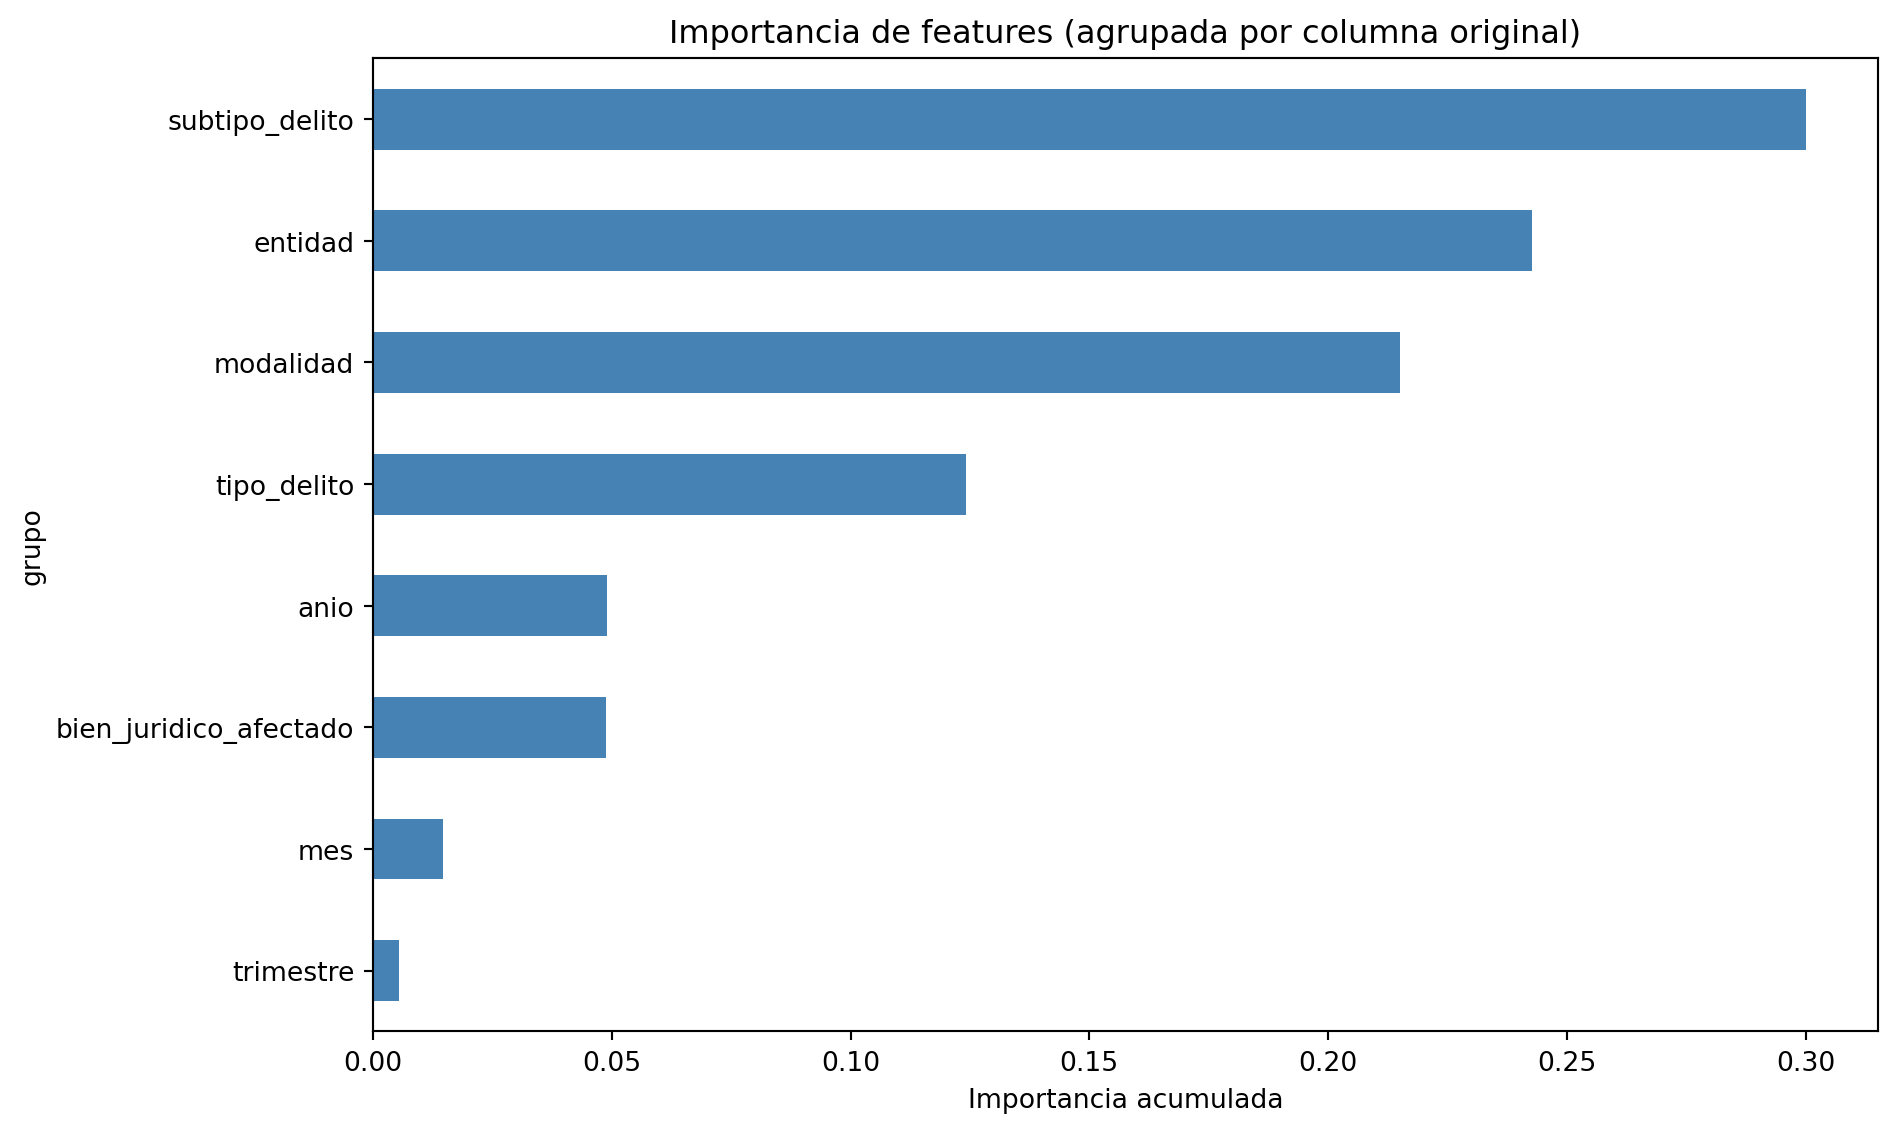
\includegraphics[width=0.75\textwidth]{imagenes/features-importance.png}
  \caption{Importancia de features agrupada por columna original}
  \label{fig:importancia-features}
\end{figure}

\subsection{Interpretación del Modelo}

El modelo obtenido tiene las siguientes implicaciones:

\begin{itemize}

\item \textbf{R$^2$ = 0.93 --- Alta capacidad predictiva.} El 93\% de la variación en la incidencia delictiva se explica por
la combinación de entidad federativa, clasificación delictiva y variables temporales. Esto indica que el
delito en México \textbf{no es un fenómeno aleatorio}: sigue patrones sistemáticos y repetibles que el modelo
puede capturar.

\item \textbf{Patrones geográficos.} Cada entidad federativa tiene un ``perfil delictivo'' distintivo. Estados como
CDMX, Estado de México y Jalisco concentran volúmenes altos en ciertas categorías, mientras que estados
como Colima o Tlaxcala muestran otras dinámicas. La feature \texttt{entidad} captura estas diferencias estructurales.

\item \textbf{Patrones por clasificación delictiva.} La jerarquía \texttt{bien\_juridico} $\rightarrow$ \texttt{tipo} $\rightarrow$ \texttt{subtipo} $\rightarrow$ \texttt{modalidad} permite
al modelo distinguir entre categorías con volúmenes muy dispares. Por ejemplo, ``homicidio'' tiene incidencias
bajas mientras que ``robo'' tiene incidencias altas; la modalidad (con/sin violencia) añade granularidad
adicional.

\item \textbf{Patrones temporales.} Las features \texttt{anio}, \texttt{mes} y \texttt{trimestre} capturan:
    \begin{itemize}
    \item \textbf{Tendencia}: incrementos o disminuciones sostenidos a lo largo de los años.
    \item \textbf{Estacionalidad}: ciclos mensuales o trimestrales (por ejemplo, incrementos en diciembre por
    temporadas vacacionales).
    \end{itemize}

\item \textbf{MAE $\approx$ 0.31 en escala log.} Para interpretar en unidades originales: $\exp(0.31) \approx 1.36$, lo que significa
que el error promedio de predicción es de aproximadamente \textbf{36\% sobre el valor real}. Para un dataset con
valores que van de decenas a miles de incidentes, esto es un margen de error razonable.

\end{itemize}

\subsubsection{Análisis gráfico}

Las gráficas de \textbf{Real vs Predicho} y de \textbf{residuales} permiten evaluar visualmente la calidad del ajuste.
En un buen modelo, los puntos deben agruparse alrededor de la diagonal en la primera gráfica, y los residuales
deben distribuirse simétricamente alrededor de cero en la segunda.

\begin{lstlisting}[language=Python, caption={Gráficas de predicciones y residuales}, label={lst:graficas-evaluacion}]
grafica_predicciones(y_test, y_pred)
grafica_residuales(y_test, y_pred)
\end{lstlisting}

\begin{figure}[H]
  \centering
  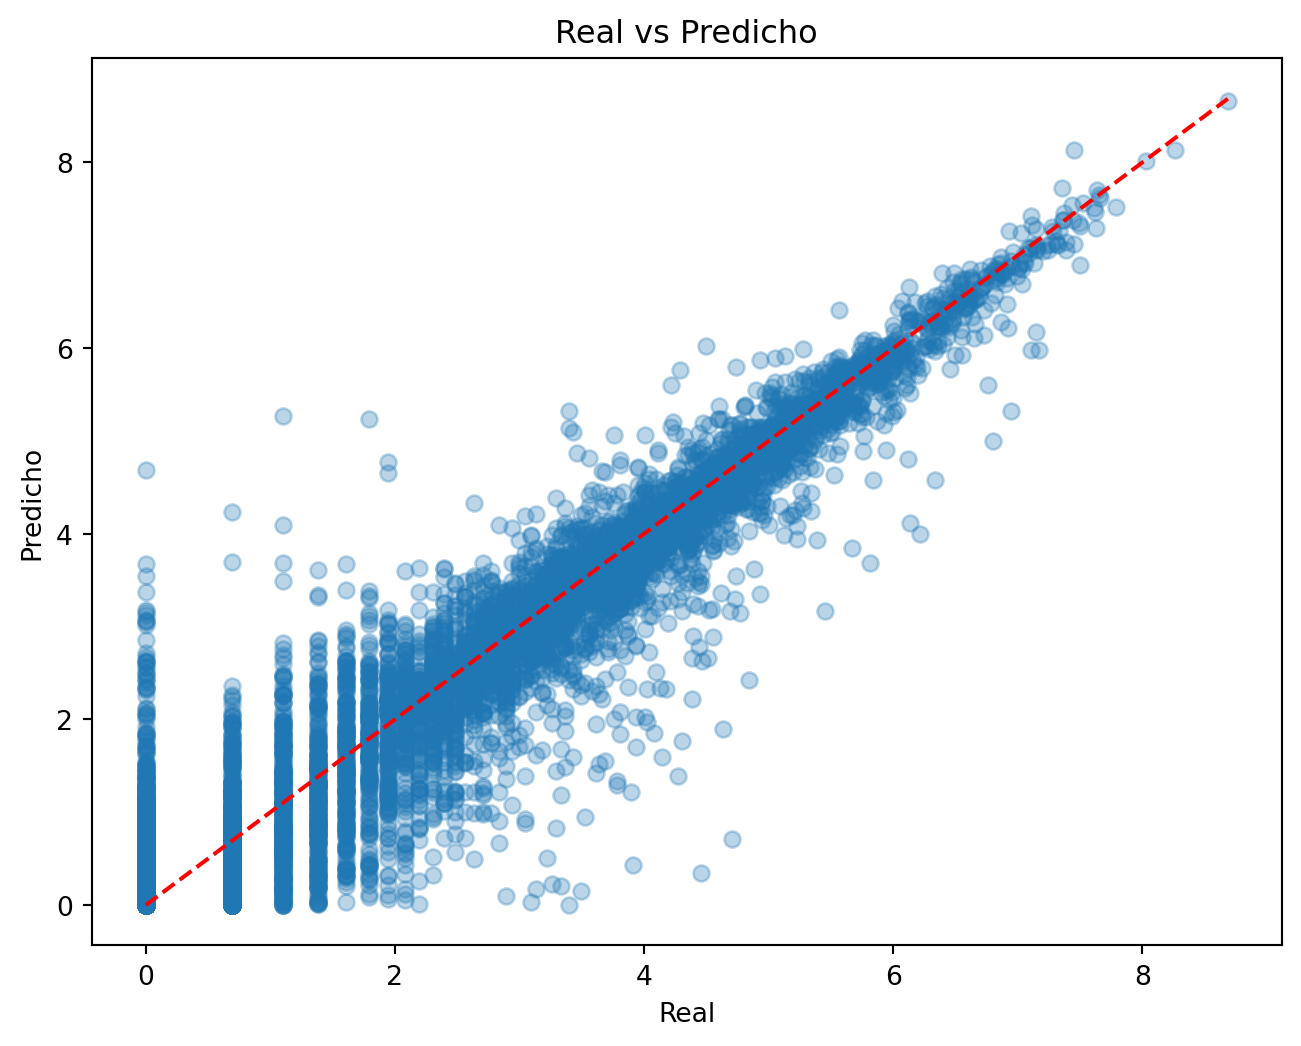
\includegraphics[width=0.7\textwidth]{imagenes/real-presaid.png}
  \caption{Gráfica de Real vs Predicho}
  \label{fig:real-vs-predicho}
\end{figure}

\begin{figure}[H]
  \centering
  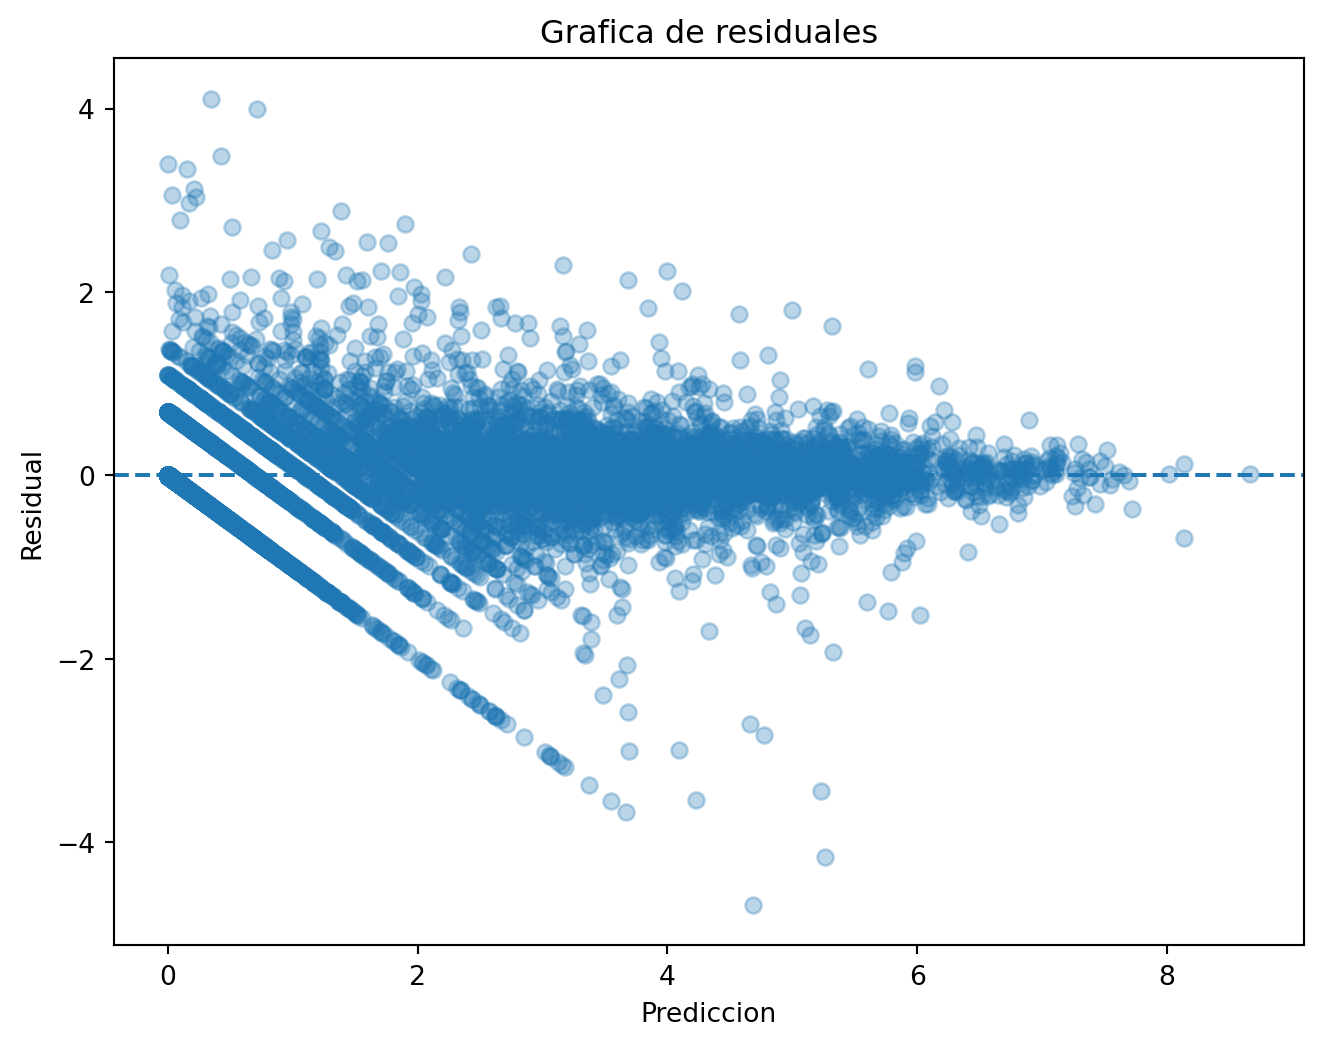
\includegraphics[width=0.7\textwidth]{imagenes/residuals.png}
  \caption{Gráfica de residuales del modelo}
  \label{fig:residuales}
\end{figure}

\subsection{Comparación con Línea Base}

Para verificar que el modelo aporta valor real, lo comparamos contra un \textbf{DummyRegressor} que simplemente
predice la media del target en cada caso. Si el Random Forest no supera significativamente a este modelo
trivial, significaría que las features elegidas no tienen poder predictivo.

\begin{lstlisting}[language=Python, caption={Comparación con DummyRegressor como línea base}, label={lst:linea-base}]
from sklearn.dummy import DummyRegressor
from sklearn.pipeline import Pipeline

baseline = Pipeline([
    ("preprocessor", preprocessor),
    ("model", DummyRegressor(strategy="mean"))
])

baseline.fit(X_train, y_train)

baseline_metricas, _ = evaluar_modelo(baseline, X_test, y_test)
display(baseline_metricas)
\end{lstlisting}

\begin{table}[ht]
  \centering
  \caption{Métricas del DummyRegressor (línea base)}
    \begin{tabular}{l l}
      \hline
      MAE & 1.719015\\
      MSE & 3.904472\\
      RMSE & 3.904472\\
      R2 & -0.000034\\
      \hline
    \end{tabular}
  \label{tab:dummy-metricas}
\end{table}

El DummyRegressor obtiene un R$^2$ $\approx$ 0 (como es esperado, ya que predecir la media no explica variación).
El Random Forest, con un R$^2$ significativamente mayor, demuestra que las features utilizadas capturan
patrones reales de la incidencia delictiva.

\subsection{Persistencia del modelo}

Finalmente, guardamos el modelo entrenado en un archivo \texttt{.joblib} para su uso futuro en predicciones o análisis
adicionales. Debido al peso del modelo final este se puede descargar desde
\href{https://drive.google.com/file/d/1p3M8-Q3r0L0FgIDpoM59of0usDTnXWrY/view?usp=sharing}{aquí}
para evitar problemas de espacio en el repositorio y de ésta página.

Sin embargo, la instrucción para guardar el modelo es la siguiente:

\begin{lstlisting}[language=Python, caption={Guardado del modelo entrenado}, label={lst:guardar-modelo}]
guardar_modelo(mejor_modelo, "../models/modelo_incidencia_delictiva.joblib")
\end{lstlisting}

\subsection{Ejemplo de Predicción}
Ahora intentaremos predecir los valores en base al modelo. Queremos predecir la incidencia delictiva de los
siguientes casos:

\begin{table}[ht]
  \centering
  \caption{Ejemplo de datos de entrada para predicción de incidencia delictiva}
  \label{tab:datos_prediccion}
  \resizebox{\textwidth}{!}{%
  \begin{tabular}{|l|l|l|l|l|c|c|c|}
    \hline
    \textbf{Entidad} & \textbf{Bien jurídico} & \textbf{Tipo de delito} & \textbf{Subtipo de delito} & \textbf{Modalidad} & \textbf{Año} & \textbf{Mes} & \textbf{Trimestre} \\ \hline
    Ciudad de México & El patrimonio & Robo & Robo de vehiculo automotor & Robo de coche de 4 ruedas Con violencia & 2026 & 5 & 1 \\ \hline
    Jalisco & La vida y la Integridad corporal & Homicidio & Homicidio doloso & Con arma de fuego & 2026 & 5 & 1 \\ \hline
  \end{tabular}%
  }
\end{table}


\begin{lstlisting}
modelo = cargar_modelo("../models/modelo_incidencia_delictiva.joblib")

# Preparación de los datos de entrada
# Las features deben coincidir con las usadas en el entrenamiento:
# - Categóricas: entidad, bien_juridico_afectado, tipo_delito, subtipo_delito, modalidad
# - Numéricas: anio, mes, trimestre

datos_ejemplo = pd.DataFrame({
    "entidad": ["Ciudad de México", "Jalisco"],
    "bien_juridico_afectado": ["El patrimonio", "La vida y la Integridad corporal"],
    "tipo_delito": ["Robo", "Homicidio"],
    "subtipo_delito": ["Robo de vehiculo automotor", "Homicidio doloso"],
    "modalidad": ["Robo de coche de 4 ruedas Con violencia", "Con arma de fuego"],
    "anio": [2026, 2026],
    "mes": [5, 5],
    "trimestre": [1, 1]
})


# El modelo predice en escala logarítmica (log1p), por lo que debemos invertir la transformación
predicciones_log = modelo.predict(datos_ejemplo)
predicciones = np.expm1(predicciones_log)  # Inversión de log1p

resultados = datos_ejemplo.copy()
resultados["incidencia_predicha"] = predicciones.round(0).astype(int)

print("Predicciones de incidencia delictiva:")
resultados
\end{lstlisting}

\begin{table}[ht]
  \centering
  \caption{Predicciones de incidencia delictiva para los casos de ejemplo}
  \label{tab:predicciones-ejemplo}
  \resizebox{\textwidth}{!}{%
  \begin{tabular}{|l|l|l|l|l|l|c|c|c|c|}
    \hline
    \textbf{Entidad} & \textbf{Bien jurídico} & \textbf{Tipo de delito} & \textbf{Subtipo de delito} & \textbf{Modalidad} & \textbf{Año} & \textbf{Mes} & \textbf{Trimestre} & \textbf{Incidencia predicha} \\ \hline
    Ciudad de México & El patrimonio & Robo & Robo de vehiculo automotor & Robo de coche de 4 ruedas Con violencia & 2026 & 5 & 1 & 50 \\ \hline
    Jalisco & La vida y la Integridad corporal & Homicidio & Homicidio doloso & Con arma de fuego & 2026 & 5 & 1 & 61 \\ \hline
  \end{tabular}%
  }
\end{table}


\subsection{Conclusiones sobre el modelo}

El modelo de Random Forest logra predecir la incidencia delictiva estatal mensual con un R$^2$ de 0.93, superando
ampliamente a la línea base (R$^2$ $\approx$ 0). Esto confirma que:

\begin{enumerate}
  \item La incidencia delictiva en México está fuertemente determinada por la ubicación geográfica, el tipo de
  delito y el momento en el tiempo. El 93\% de la variación en la incidencia delictiva se explica por la
  combinación de ubicación geográfica, clasificación delictiva y momento en el tiempo. Esto descarta la
  hipótesis de que la criminalidad sea un fenómeno aleatorio o caótico: sigue patrones estables y recurrentes
  que un modelo de aprendizaje automático puede capturar con alta precisión.

  \item Las variables utilizadas (entidad, clasificación delictiva, año/mes/trimestre) son suficientes para
  construir un modelo predictivo robusto. Sobre todo con estos datos más recientes, ya que el EDA mostró que
  la incidencia delictiva no ha decrecido entre 2015 y 2025, con un incremento notable desde 2022. Además,
  se observa estacionalidad: los picos se concentran entre marzo y junio en los últimos años (antes eran
  mayo-agosto). El modelo captura estos ciclos a través de las features \texttt{anio}, \texttt{mes} y \texttt{trimestre}, lo
  que permite identificar cuándo ocurren los periodos de mayor riesgo.

  \item Los patrones delictivos son \textbf{estables y predecibles} en condiciones normales, lo cual es relevante
  para la planeación de políticas de seguridad. En particular, la clasificación delictiva es el predictor
  más potente, ya que la jerarquía \texttt{bien\_juridico} $\rightarrow$ \texttt{tipo} $\rightarrow$ \texttt{subtipo} $\rightarrow$ \texttt{modalidad} permite distinguir entre
  categorías con volúmenes drásticamente diferentes. Como se vio en el EDA, Robo es el delito más reportado,
  pero la modalidad (con violencia, sin violencia, de vehículo automotor, etc.) añade granularidad que el
  modelo aprovecha para hacer predicciones más precisas.
\end{enumerate}

\subsubsection{Limitaciones}

\begin{itemize}
  \item El modelo aprende patrones históricos y no puede predecir anomalías como pandemias, crisis o cambios de
  política pública. El caso de 2020 (valores inusualmente bajos por COVID-19) es un ejemplo de evento que
  el modelo no anticiparía.
  \item Los datos dependen de denuncias ante el Ministerio Público, por lo que zonas con bajo reporte pueden tener
  valores artificialmente bajos.
  \item El modelo identifica correlaciones, no causalidades. Por ejemplo, saber que CDMX tiene alta incidencia
  de robo no explica por qué ocurre, lo cual es algo ajeno a lo que se realiza en este proyecto.
\end{itemize}

    \input{contenido/clustering.tex}
    \section{Conclusiones}

El análisis integral de la incidencia delictiva en México entre 2015 y 2025 demuestra que la criminalidad
no es un fenómeno aleatorio, sino que sigue patrones sistemáticos determinados por la ubicación geográfica,
la clasificación delictiva y las condiciones temporales. El modelo predictivo de Random Forest alcanzó un R$^2$
de 0.93, lo que confirma que el 93\% de la variación en la incidencia delictiva puede explicarse mediante la
entidad federativa, el tipo de delito y variables como año, mes y trimestre. Esto descarta la hipótesis de
caos o impredecibilidad: los patrones delictivos son estables y recurrentes bajo condiciones normales, lo
cual es relevante para la planeación de políticas públicas de seguridad.

El análisis exploratorio reveló que la incidencia delictiva no ha disminuido en más de una década, con un
incremento notable a partir de 2022, y que los picos se concentran entre marzo y junio en los años recientes.
El robo es el delito más reportado a nivel nacional, mientras que estados como el Estado de México, CDMX y
Jalisco lideran en volumen absoluto. El clustering identificó cuatro perfiles delictivos claramente
diferenciados: un perfil de violencia contra las personas (sur y centro-pacífico), uno patrimonial
(áreas urbanas de alta densidad), uno familiar y de libertad personal, y uno diversificado. Estos perfiles
permiten entender que cada entidad federativa enfrenta dinámicas criminales distintas que requieren
estrategias de prevención diferenciadas.

Entre las limitaciones del proyecto destacan que el modelo aprende de patrones históricos y no puede
anticipar eventos anómalos como pandemias o crisis políticas, y que los datos dependen de denuncias
ante el Ministerio Público, lo que puede generar subreporte en ciertas zonas. Además, el modelo identifica
correlaciones, no causalidades: saber que CDMX tiene alta incidencia de robo no explica por qué ocurre.

No obstante, el proyecto logra su objetivo principal de proporcionar una herramienta analítica que permite
identificar los delitos más probables por estado y predecir su incidencia, ofreciendo una base sólida para
la toma de decisiones en materia de seguridad pública.
\end{spacing}

\newpage
\nocite{*}
\printbibliography
\end{document}
